\documentclass[sigconf, anonymous, review]{acmart}

%% For camera-ready (after acceptance), change the line above to:
%% \documentclass[sigconf]{acmart}

\AtBeginDocument{%
  \providecommand\BibTeX{{%
    Bib\TeX}}}

\graphicspath{{images/}}

%% Rights management information.
%%\setcopyright{acmlicensed}
%%\copyrightyear{2025}
%%\acmYear{2025}
%%\acmDOI{XXXXXXX.XXXXXXX}
%%\acmConference[CHI '25]{Proceedings of the 2025 CHI Conference on Human Factors in Computing Systems}{April 26--May 1, 2025}{Yokohama, Japan}
%%\acmISBN{978-1-4503-XXXX-X/2025/04}

\begin{document}

\title{MobileAgents: Designing and Evaluating a Mobile Multimodal Interface for Controlling Personal AI Agents On the Go}

\author{Anonymous Author}
\email{anonymous@university.edu}
\affiliation{%
  \institution{Anonymous University}
  \city{City}
  \country{Country}}

\renewcommand{\shortauthors}{Anonymous}

\begin{abstract}
People increasingly rely on personal AI agents---for research, messaging, scheduling---but controlling these agents away from a desktop is cumbersome: typing complex instructions on a phone is slow, and existing orchestration frameworks offer no end-user interface at all. We designed MobileAgents, a mobile-first platform where users bring their own AI agents and control them on the go through text, voice, and camera input. An LLM orchestrator decomposes multimodal requests into a dependency-aware plan across the user's personal agent pool, and a live DAG streams execution progress. The architecture is agent-agnostic: any agent can be registered with its role and tools at runtime---no code changes required. To study how much of this orchestration to reveal, we compared three transparency configurations---Black Box, Plan Preview, and Full Transparency---in a mixed-methods study with 10 participants (think-aloud, surveys, interviews). Plan Preview offered the best balance of trust and efficiency for mobile use; voice and image input were valued for on-the-go scenarios but required consent gating. We discuss value trade-offs, automation bias risks, and design implications for mobile multimodal agent control.
\end{abstract}

\begin{CCSXML}
<ccs2012>
 <concept>
  <concept_id>10003120.10003121.10003129</concept_id>
  <concept_desc>Human-centered computing~Interactive systems and tools</concept_desc>
  <concept_significance>500</concept_significance>
 </concept>
 <concept>
  <concept_id>10003120.10003121.10003125.10011752</concept_id>
  <concept_desc>Human-centered computing~Empirical studies in HCI</concept_desc>
  <concept_significance>500</concept_significance>
 </concept>
</ccs2012>
\end{CCSXML}

\ccsdesc[500]{Human-centered computing~Interactive systems and tools}
\ccsdesc[500]{Human-centered computing~Empirical studies in HCI}

\keywords{multimodal interaction, agent orchestration, transparency, human-in-the-loop, trust, human--AI interaction}

\maketitle

%% ============================================================
\section{Introduction: Use Case and Goals}
%% ============================================================

People increasingly assemble personal toolkits of AI agents---one for paper search, another for drafting, another for team messaging---but controlling these agents is tethered to the desktop. Typing multi-step instructions into a terminal or notebook is impractical when walking between meetings, commuting, or working from a phone. Current orchestration frameworks (CrewAI, LangGraph, AutoGen) compound this problem: they are developer-facing APIs with no end-user interface at all, let alone a mobile one. The demand for mobile agent control is real: Clawdbot~\cite{Clawdbot2025}, an open-source autonomous AI agent that operates via messaging platforms (WhatsApp, Telegram, Slack), grew to an estimated 300,000--400,000 users within months of its 2025 launch by letting people delegate tasks---reading emails, managing calendars, deploying code---from their phone. Yet Clawdbot operates as a single opaque agent with broad permissions and no plan preview, approval gates, or transparency into what it will do before it acts, drawing scrutiny from security researchers over misconfigured instances accessing sensitive services. AI systems always involve value-laden choices, even when they appear purely technical~\cite{SadekMougenot2025}; orchestration platforms are no exception, yet they offer no mechanism for users to inspect plans, intervene before irreversible actions, or issue commands via voice or camera. Shneiderman~\cite{Shneiderman2020} argues that human-centred AI must be simultaneously reliable, safe, and trustworthy. Amershi et al.~\cite{Amershi2019} distil 18 guidelines for human--AI interaction, including ``make clear what the system can do'' (G1) and ``support efficient correction'' (G2); agent orchestration platforms violate nearly all of them by design, since they have no user-facing layer at all.

We designed \textbf{MobileAgents}, a mobile-first platform that lets users \emph{bring their own AI agents} and control them on the go through text, voice, and image input. The architecture is \textbf{agent-agnostic}: any agent can be registered at runtime by defining its role, tools, and metadata---no code changes to the orchestration or UI layer. An LLM orchestrator decomposes multimodal requests into a dependency-aware execution plan across the user's personal agent pool, and a live directed acyclic graph (DAG) streams progress in real time. The platform ships with five demo agents (ArXiv, Proposal, Wikipedia, Slack, Semantic Scholar), but these are illustrative; the value proposition is that users plug in \emph{whatever agents matter to them} and manage them from their phone through whichever modality suits the moment---voice while walking, a photo of a whiteboard in a meeting, or text at a desk.

A multi-agent orchestrator is a particularly challenging AI \emph{design material}: its behaviour is emergent (plans depend on which agents are registered and what the LLM decides), data-dependent (multimodal inputs shape plans unpredictably), and opaque (multiple agents execute in parallel behind the scenes). Recent scaling studies show that multi-agent coordination amplifies errors---centralized architectures amplify errors 4.4$\times$ compared to 17.2$\times$ for independent agents~\cite{Kim2025}---motivating our centralized orchestrator design. Capel and Brereton~\cite{Capel2023} map the HCAI research landscape and identify transparency, user agency, and contextual awareness as under-explored in agentic systems. The central design question is therefore \emph{how much} of this internal orchestration to expose on a small screen. We operationalise this as three configurable \textbf{transparency modes}---Black Box, Plan Preview, and Full Transparency---and evaluate their impact on users.

\textbf{Stakeholders and values.} We adopted the tripartite VSD methodology~\cite{Friedman2002, Friedman2017}---conceptual, empirical, and technical investigations---as our overarching design framework. In the \emph{conceptual investigation}, we identified direct and indirect stakeholders following Friedman et al.'s~\cite{Friedman2017} stakeholder analysis method and performed a \emph{value source analysis} to distinguish project-endorsed values (usability, performance) from stakeholder-held values that might diverge from designer assumptions~\cite{Friedman2017}. Primary stakeholders: researchers and professionals who maintain personal agent pools and need mobile access. Secondary: collaborators who receive agent-generated outputs (e.g., Slack messages sent on the user's behalf). Tertiary: IT administrators concerned with data governance when agents act across services. We then conducted an \emph{empirical investigation} using value-oriented semi-structured interviews~\cite{Friedman2017}: informal conversations with four graduate students, structured as participatory inquiry. Participatory design, rooted in Scandinavian workplace democracy movements of the 1970s, holds that people affected by a technology should have a voice in shaping it~\cite{Sanders2008}---not merely as consultees but as genuine collaborators. This co-design orientation ensured that values emerged from lived experience rather than designer assumptions. Three core values surfaced: \textbf{V1~Efficiency} (``I want to fire off a request from my phone and get a result---don't slow me down''), \textbf{V2~Control} (``I need to verify before it sends anything on my behalf''), and \textbf{V3~Privacy} (``I don't want my voice recorded or images stored''). These values are in tension---V1 favours opacity, V2 demands visibility, V3 constrains which modalities feel safe in public---a pattern Friedman et al.~\cite{Friedman2017} call \emph{value tensions}, which drive design trade-offs rather than admit simple resolution. This motivates our research question.

%% ============================================================
\section{Methods: System Design and Implementation}
%% ============================================================

\subsection{Prototype Overview}

\begin{figure*}[t]
  \centering
  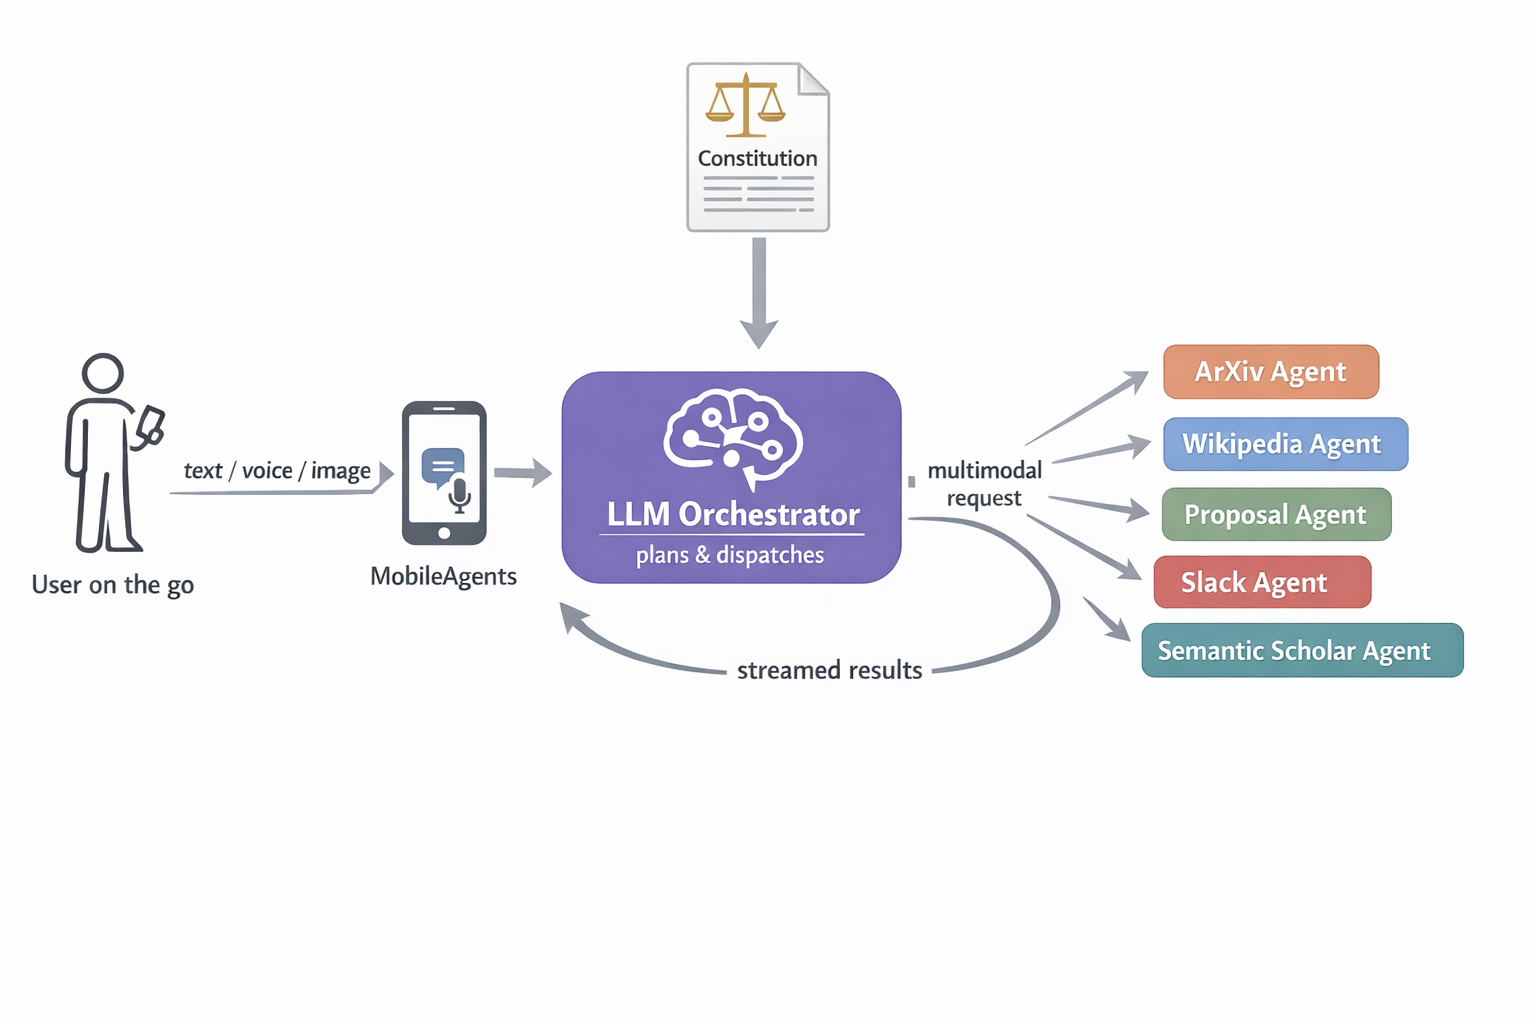
\includegraphics[width=0.92\textwidth]{flow}
  \caption{MobileAgents system overview. A user on the go issues a multimodal request (text, voice, or image) from their phone. The LLM Orchestrator decomposes it into a dependency-aware plan and dispatches tasks across the user's personal agent pool (ArXiv, Wikipedia, Proposal, Slack, Semantic Scholar). Results stream back to the mobile client in real time.}
  \Description{Architecture flow diagram: person labeled User on the go sends text/voice/image to a phone labeled MobileAgents, which forwards a multimodal request to a purple LLM Orchestrator box that fans out to five colored agent boxes, with a streamed results arrow returning to the phone.}
  \label{fig:flow}
\end{figure*}

MobileAgents is a fully functional prototype (Figure~\ref{fig:flow}; full architecture in Appendix~\ref{app:architecture}--\ref{app:structure}). The client is built in React with Konsta UI for mobile components as a Progressive Web App. The backend is a FastAPI server and communicates with the client through REST APIs and Server-Sent Events. The Orchestrator and demo agents are implemented with CrewAI and powered by GPT-4.1.



\begin{figure*}[t]
  \centering
  \begin{minipage}[t]{0.3\textwidth}
    \centering
    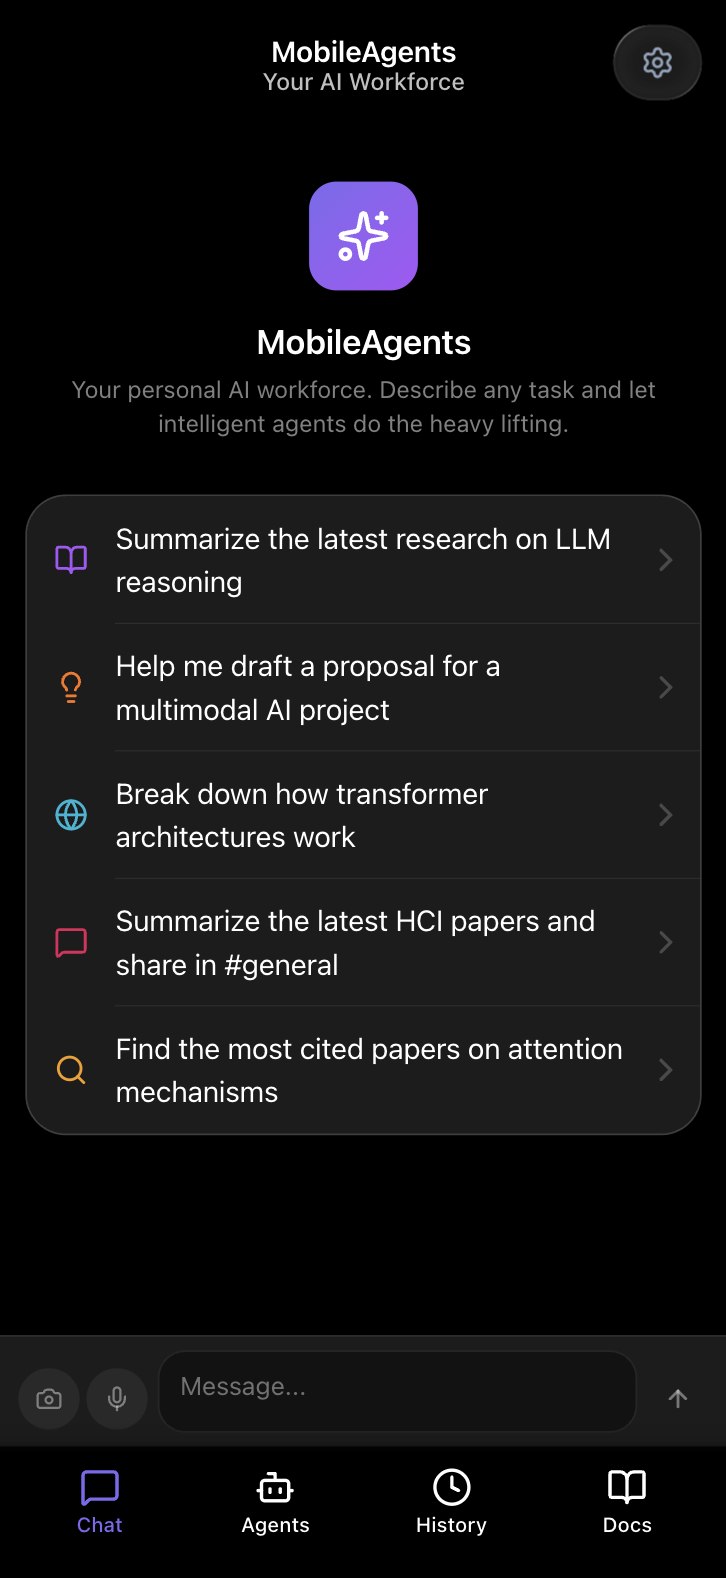
\includegraphics[height=6.5cm]{multi_modal}\\[2pt]
    \small (a) Multimodal mode
  \end{minipage}
  \hfill
  \begin{minipage}[t]{0.3\textwidth}
    \centering
    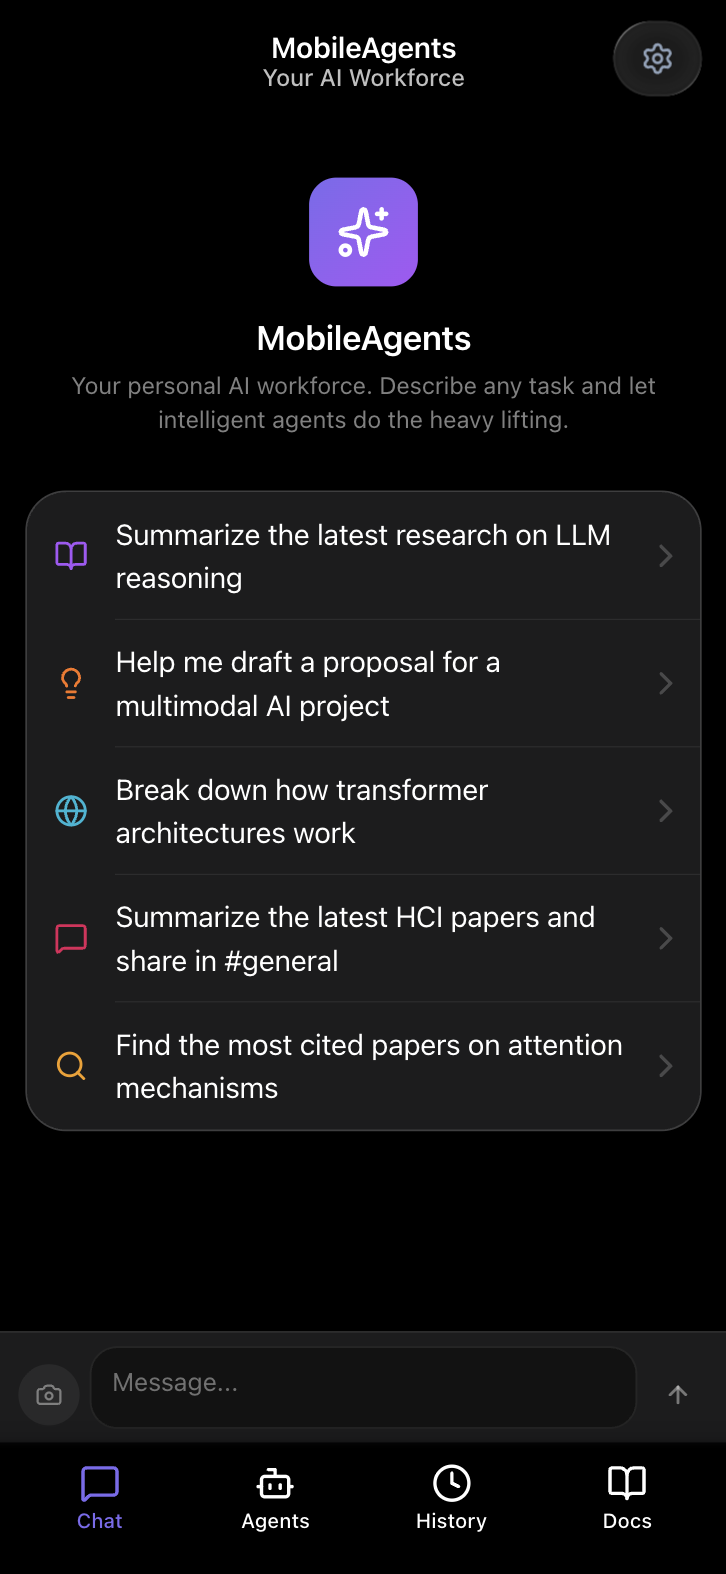
\includegraphics[height=6.5cm]{text+images}\\[2pt]
    \small (b) Text + Images mode
  \end{minipage}
  \hfill
  \begin{minipage}[t]{0.3\textwidth}
    \centering
    
\includegraphics[height=6.5cm]{voice_only}\\[2pt]
    \small (c) Voice-only mode (listening)
  \end{minipage}
  \caption{MobileAgents input modes. (a)~Multimodal (b)~Text + Images. (c)~Voice-only}
  \Description{Three mobile screenshots: (a) dark-themed chat home with multimodal input bar; (b) same screen with camera-only input; (c) full-screen voice recording with red microphone button and Listening indicator.}
  \label{fig:chat}
\end{figure*}

\subsection{Modality Support}

Users interact with three modalities optimized for mobile that can be configured in settings (Figure~\ref{fig:chat}). \textbf{Multimodal} supports text, images, and speech, and responds with text and visualizations, with an optional text-to-speech button. \textbf{Text and Image} mode supports text and images as input and responds with text and visualizations. \textbf{Voice-only} mode is unique as it supports only speech input and responds only in speech. While this enables convenience, it also restricts visualization, planning, and approval, and is designed to be more concise. The orchestrator decomposes the request into a dependency graph of tasks and assigns them to the corresponding agents. Responses are streamed in real-time updates via Server-Sent Events.

\subsection{Design Rationale}

The \emph{technical investigation}~\cite{Friedman2002, Friedman2017} translated values into design requirements. We drew on Amershi et al.'s~\cite{Amershi2019} 18 HAI guidelines, Shneiderman's~\cite{Shneiderman2020} HCAI framework, and van de Poel's~\cite{vanDePoel2013} value-to-requirement hierarchy. Umbrello and van de Poel~\cite{Umbrello2021} demonstrate that VSD can be systematically mapped onto AI systems by treating values as first-class design constraints; Sadek et al.~\cite{Sadek2024CHI} provide concrete guidelines for integrating VSD into responsible AI toolkits, recommending that value--design mappings be documented and traceable. We followed this approach, mapping each stakeholder value to a concrete design implication and tracing it to specific HAI guidelines:

\begin{itemize}
  \item \textbf{V1$\rightarrow$D1:} Black Box mode for speed-oriented users (no plan, no graph, auto-execute). This prioritises Amershi et al.'s G5 (``match relevant social norms'') for users who expect instant results on mobile.
  \item \textbf{V2$\rightarrow$D2:} Plan Preview and Full Transparency modes with approval gates before irreversible actions. This operationalises G1 (``make clear what the system can do''), G2 (``support efficient correction''), and G11 (``make clear why the system did what it did'')~\cite{Amershi2019}. Jerry et al.~\cite{Jerry2025} argue for \emph{human oversight-by-design}: embedding human judgment throughout the AI pipeline via risk detection and escalation, rather than appending it as a final review step. Our checkpoint gates realise this principle---they are distributed throughout the execution graph, not just at the end. Shneiderman's~\cite{Shneiderman2020} audit trail principle is realised through the live DAG, which provides a visual record of every agent action.
  \item \textbf{V3$\rightarrow$D3:} Consent-gated multimodality---camera and microphone trigger a privacy dialog on first use explaining that data is sent to OpenAI; consent is revocable. This addresses G16 (``convey the consequences of user actions'')~\cite{Amershi2019} and Shneiderman's safety requirement.
\end{itemize}

\subsection{Persona, Tone, and Agent Customisation}

We designed an AI orchestrator persona (full text in Appendix~\ref{app:backstories}): a concise research librarian that uses uncertainty-aware language (addressing Amershi et al.'s G13: ``mitigate social biases''~\cite{Amershi2019} by avoiding overconfident claims), prefers parallel execution, and never claims authority over institutional policy. Critically, the orchestrator's system prompt includes a user-editable ``constitution'' field---free-text guidelines that are appended at planning time. This lets users shape \emph{how} their personal agent pool is coordinated (e.g., ``always run ArXiv and Semantic Scholar in parallel,'' ``never send Slack messages without showing me a draft first''). The constitution operationalises co-design's core tenets~\cite{Sanders2008}: empowerment (giving users control over decisions that affect them), mutual learning (users discover orchestration possibilities while the system learns user preferences), and democratisation of design (opening up AI coordination rules that are normally developer-only). Sanders and Stappers~\cite{Sanders2008} call this moving users from ``passive consumer'' to ``co-creator.'' It also operationalises Amershi et al.'s G15 (``provide global controls'')~\cite{Amershi2019} and Shneiderman's~\cite{Shneiderman2020} principle that users should be able to set automation boundaries. Each worker agent can be enabled, disabled, inspected, or deleted from the Agents tab, giving users full control over which agents are available for orchestration. Sadek et al.'s~\cite{Sadek2025IJHCI} value-sensitive conversational agent co-design framework demonstrates that co-designing agent values with end users yields more contextually appropriate behaviour; their comprehensive review of co-design methods for conversational agents~\cite{Sadek2023} further recommends embedding value elicitation throughout iterative design cycles rather than treating it as a one-off activity. Our constitution mechanism extends this idea by making value alignment an ongoing, user-driven activity embedded in the runtime system itself. This also embodies VSD's principle of \emph{co-evolution of technology and social structure}~\cite{Friedman2017}: as users write new constitution rules, both the technology's behaviour and the social practices around it evolve together.

\subsection{Execution Control}
\label{sec:configs}

The three execution control settings are \textbf{Black Box}, \textbf{Plan Preview}, and \textbf{Full Transparency} (Figure~\ref{fig:configs}). Black Box enables the orchestrator and agents to execute tasks autonomously. Plan Preview proposes a plan that requires approval. Full Transparency proposes a plan that requires approval and embeds an execution graph that updates in real time as the multi-agent system executes tasks, providing full visibility into the system's operation. Transparency into agents is available through the agent tab, where users can view each agent, their available tools, and system prompts.

\begin{table}[h]
  \caption{The three transparency configurations compared.}
  \label{tab:transparency}
  \small
  \begin{tabular}{p{0.18\columnwidth} p{0.72\columnwidth}}
    \toprule
    Configuration & What the user sees and can do \\
    \midrule
    C1: Black Box & Query in, final answer out. Agents auto-execute. \\
    C2: Plan Preview & Orchestrator's task plan. \\
    C3: Full Transparency &  Plan with a real-time graph, and checkpoint approvals \\
    \bottomrule
  \end{tabular}
\end{table}

\begin{figure*}[t]
  \centering
  \begin{minipage}[t]{0.22\textwidth}
    \centering
    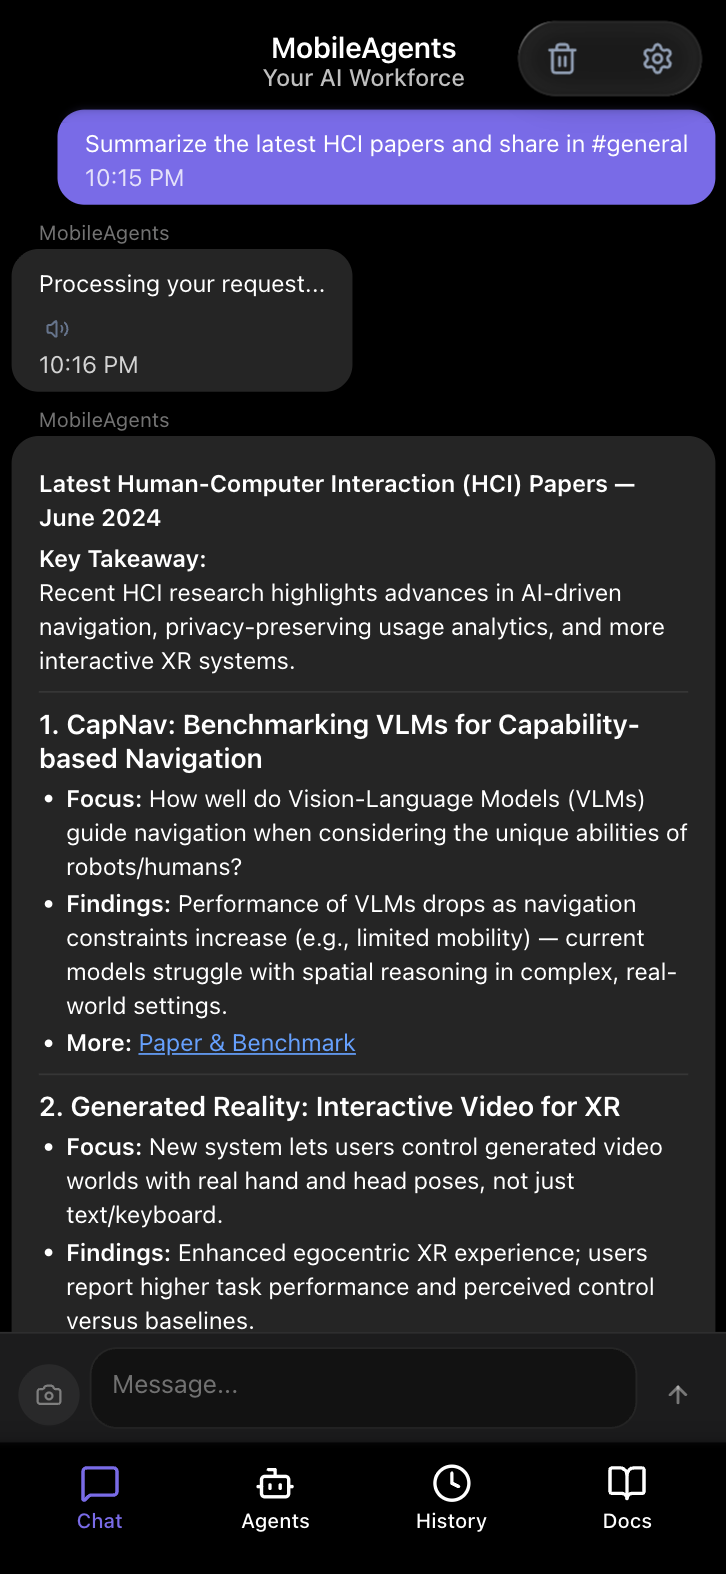
\includegraphics[height=6.5cm]{blackbox}\\[2pt]
    \small (a) C1: Black Box
  \end{minipage}
  \hfill
  \begin{minipage}[t]{0.22\textwidth}
    \centering
    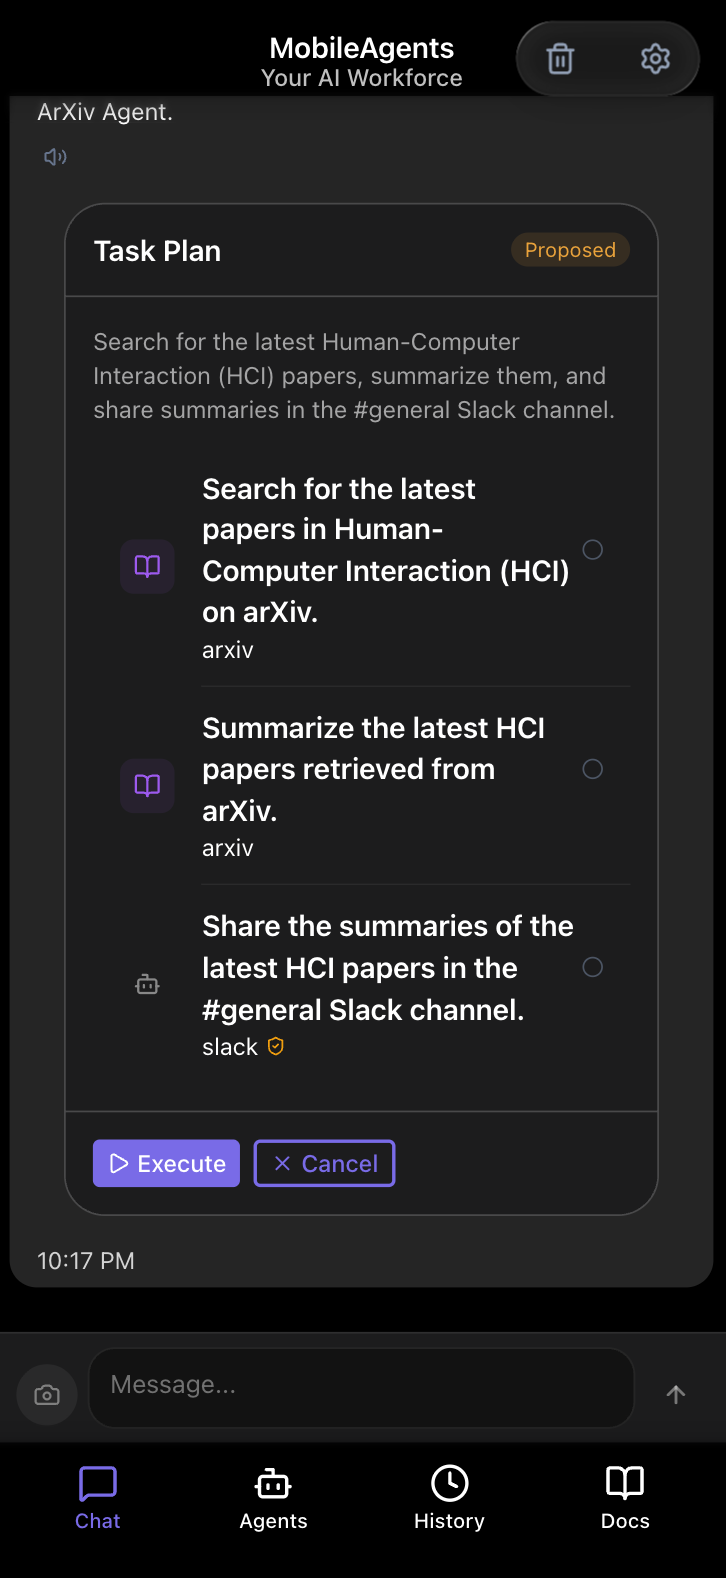
\includegraphics[height=6.5cm]{task_plan}\\[2pt]
    \small (b) C2: Plan Preview
  \end{minipage}
  \hfill
  \begin{minipage}[t]{0.22\textwidth}
    \centering
    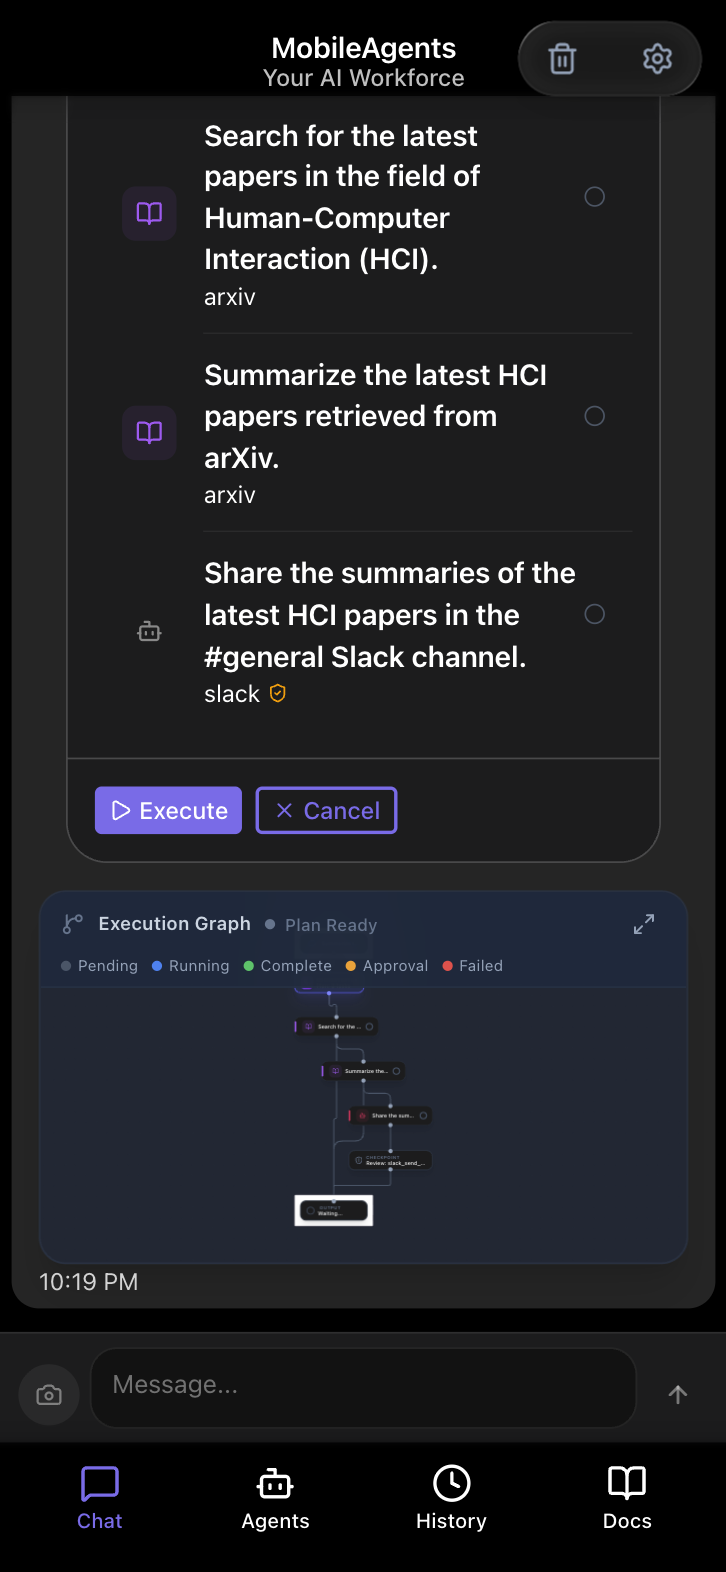
\includegraphics[height=6.5cm]{full_control}\\[2pt]
    \small (c) C3: Full Transparency
  \end{minipage}
  \hfill
  \begin{minipage}[t]{0.22\textwidth}
    \centering
    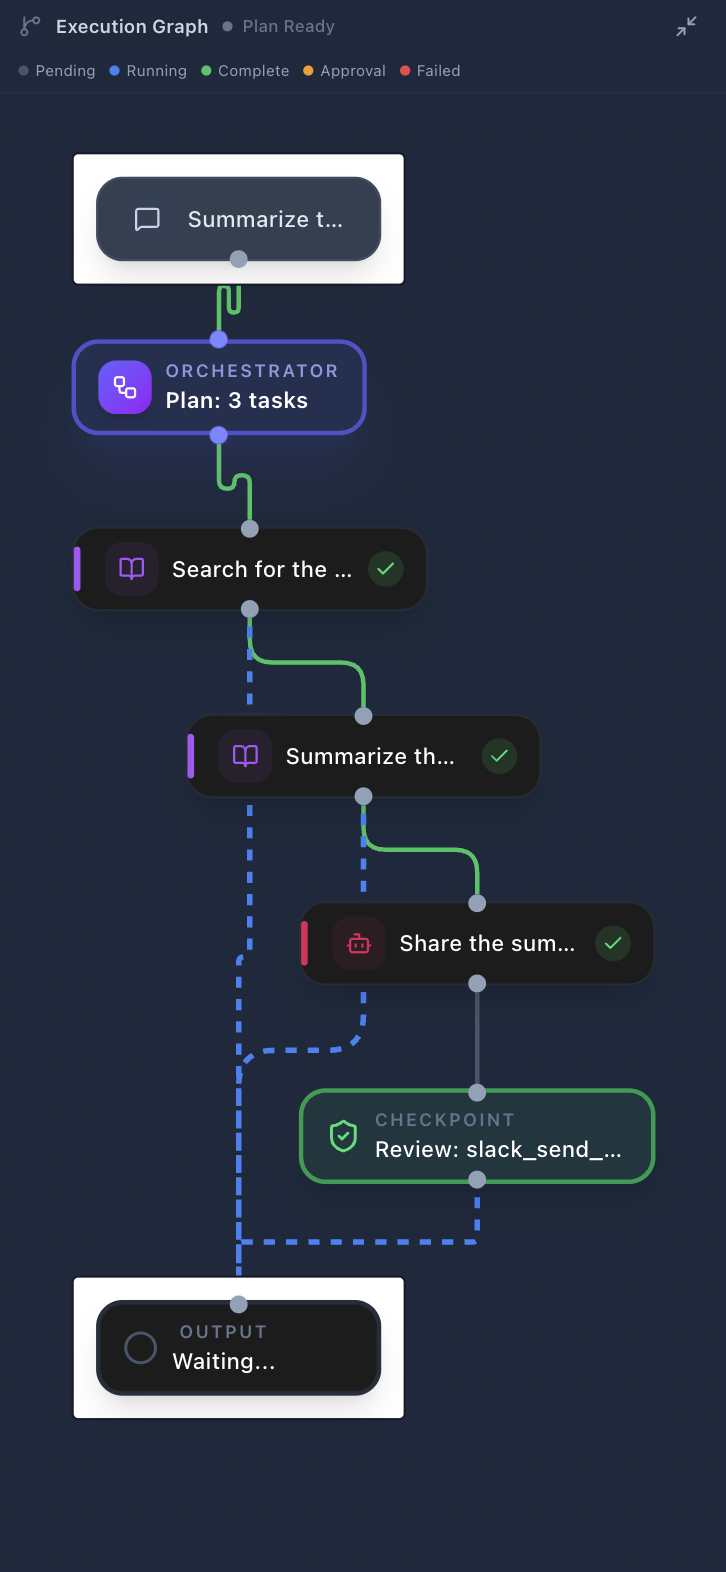
\includegraphics[height=6.5cm]{execution_graph}\\[2pt]
    \small (d) Live DAG (C3 detail)
  \end{minipage}
  \caption{The three transparency configurations and the C3 graph. (a)~Black Box (b)~Plan Preview (c)~Full Transparency (d)~Graph Close-up of Full Transparency}
  \Description{Four panels: Black Box output screen, Plan Preview card, Full Transparency with embedded DAG, and a close-up DAG showing orchestrator, agent, checkpoint, and output nodes.}
  \label{fig:configs}
\end{figure*}

These configurations follow Shneiderman's~\cite{Shneiderman2020} framework of efficiency and control trade-off. C1 has high autonomy and low human control. C3 has at low automation with high human control. C2 is in between.

\subsection{Agentic Control Settings}

Additional control is given to the user through agentic settings. The Orchestrator takes in a Constitution inspired by Anthropic's Constitutions~\cite{Anthropic2023}. This constitution provides instructions to guide orchestration logic, planning, and response stylization. It is editable from the UI and does not require system updates. Furthermore, individual agents can be turned on or off, allowing users to control which agents are accessible to the orchestrator. This functionality works in tandem with the execution control settings discussed before to enable users to manage risk. For example, a high-risk agent can be deployed with full transparency mode, and a low-risk one can be used effectively in Black Box.

\subsection{Accessibility and Inclusion}

HCAI demands inclusivity across age, language, culture, and ability levels~\cite{Capel2023}. MobileAgents supports English, Chinese, Arabic with full RTL layout, and Bulgarian. It has dark, light, and auto color themes. Icon buttons contain ARIA labels. Users with different abilities and devices can utilize the product through multimodal inputs of text, voice, and images, with neither being a point-of-failure. The design was chosen with personalization in mind and to not impose a single interaction pattern.

%% ============================================================
\section{Methods: Research Question, Evaluation Methods, and Metrics}
%% ============================================================

\subsection{Research Question}

\textbf{RQ:} How does the level of transparency in a multi-agent AI orchestrator affect user trust, perceived control, and task efficiency?

\subsection{Study Design}

We conducted a within-subjects study: each participant used all three configurations in counterbalanced order (Latin square) to control for learning effects. To simulate realistic mobile, on-the-go scenarios, participants completed tasks using different modalities: (T1)~type a text query to find and compare two recent papers on a given topic, (T2)~photograph a printed paper abstract with the camera and ask the system to find related work and draft a proposal, and (T3)~use voice input to dictate a request to summarise results and send them to a Slack channel. These tasks exercise the full multimodal range and span the agent pool (ArXiv, Wikipedia, Proposal, Slack). Tasks were matched in complexity and counterbalanced across configurations.

\subsection{Participants}

We recruited 10 participants (6 male, 4 female; ages 22--28, $M=24.3$) from a university graduate programme. All had experience with LLM-based tools but none had used multi-agent systems. Participation was voluntary.

\subsection{Evaluation Methods}

Traditional usability metrics (task completion, click-through rates) are insufficient for AI systems, where evaluation must also capture trust calibration, mental model accuracy, perceived agency, and error tolerance~\cite{Buçinca2020}. We therefore used a mixed-methods approach---essential for capturing the full AI experience---with three methods, all directly involving users:

\begin{enumerate}
  \item \textbf{Think-aloud sessions} (user-involving, qualitative): Participants verbalised their thoughts while completing tasks. Sessions were screen-recorded and the researcher took timestamped notes on hesitations, errors, and interaction breakdowns. This method surfaces \emph{in-situ} mental model accuracy and trust calibration~\cite{Buçinca2020}---whether users' expectations of what the system will do match what it actually does---which surveys alone cannot capture.
  \item \textbf{Post-task survey} (user-involving, quantitative): After each configuration, participants rated 7-point Likert items for \emph{trust}, \emph{perceived control}, and \emph{satisfaction} (full items in Appendix~\ref{app:survey}). Trust items draw on Jian et al.'s~\cite{Jian2000} empirically validated Trust in Automation scale, which measures trust as a function of perceived reliability and predictability. Usability items draw on Brooke's~\cite{Brooke1996} System Usability Scale. These constructs are well suited because our research question centres on how transparency mediates trust and control.
  \item \textbf{Semi-structured interview} (user-involving, qualitative): After all three conditions, a 10-minute interview explored preferences, trust calibration, privacy concerns, and suggestions (questions in Appendix~\ref{app:interview}). Interview data was analysed alongside think-aloud transcripts.
\end{enumerate}

\subsection{Metrics}

\begin{enumerate}
  \item \textbf{Trust, perceived control, and satisfaction} (Likert, 1--7): from the post-task survey, grounded in Jian et al.'s~\cite{Jian2000} trust dimensions.
  \item \textbf{Task completion time} (seconds): measured from first input to final system response---an objective efficiency measure to complement subjective ratings.
  \item \textbf{Qualitative themes}: from Braun and Clarke's~\cite{Braun2012} reflexive thematic analysis of think-aloud transcripts and interview responses. We followed their six-phase process (familiarisation, coding, theme generation, review, definition, write-up) to identify patterns across participants.
\end{enumerate}

%% ============================================================
\section{Results}
%% ============================================================

\subsection{Quantitative Findings}

Table~\ref{tab:results} summarises survey scores and task times across the three configurations. Given the small sample ($N=10$), we report descriptive statistics rather than inferential tests.

\begin{table}[h]
  \caption{Mean (SD) survey scores (1--7 Likert) and task completion time (seconds) per configuration.}
  \label{tab:results}
  \small
  \begin{tabular}{p{0.22\columnwidth} p{0.17\columnwidth} p{0.17\columnwidth} p{0.25\columnwidth}}
    \toprule
    Metric & C1: Black Box & C2: Plan Preview & C3: Full Transp. \\
    \midrule
    Trust          & 3.8 (1.2) & 5.6 (0.8) & 6.1 (0.7) \\
    Control        & 2.4 (1.1) & 5.2 (0.9) & 6.3 (0.6) \\
    Satisfaction   & 5.1 (1.0) & 5.8 (0.7) & 5.4 (1.1) \\
    Time (s)       & 68 (14)   & 89 (18)   & 112 (22)  \\
    \bottomrule
  \end{tabular}
\end{table}

Trust and control increased monotonically with transparency, consistent with Shneiderman's~\cite{Shneiderman2020} argument that human oversight and automation are not zero-sum. However, satisfaction peaked at C2 (Plan Preview): C3's additional graph detail improved control but introduced cognitive overhead, with three participants describing the live DAG as ``a lot to take in''---a tension Amershi et al.~\cite{Amershi2019} anticipate in G3 (``time services based on context''), suggesting that mobile contexts demand lighter-weight feedback. Task time increased with transparency due to plan inspection and checkpoint approval steps.

\subsection{Qualitative Themes}

Reflexive thematic analysis of think-aloud and interview data yielded four themes:

\textbf{Theme 1: Intervention trumps observation.} Participants valued the ability to \emph{act}---approving, rejecting, or modifying a plan---more than passively watching execution. One participant noted: ``Seeing the graph is cool, but what actually makes me trust it is that I can stop it before it sends the Slack message.'' This directly validates Amershi et al.'s~\cite{Amershi2019} G2 (``support efficient correction'') and G18 (``support efficient dismissal'')---users trusted the system not because it was accurate, but because they could \emph{intervene}. This also aligns with Parasuraman and Riley's~\cite{Parasuraman1997} observation that trust in automation depends on the user's perceived ability to override it. The finding is particularly important given Pappu et al.'s~\cite{Pappu2025} recent result that unsupervised multi-agent teams \emph{degrade} expert performance by up to 37.6\% through ``integrative compromise''---averaging expert and non-expert agent views rather than appropriately weighting expertise. Human intervention may be essential not merely for trust, but to prevent multi-agent consensus from diluting output quality.

\textbf{Theme 2: Plan Preview as the `sweet spot.'} 7 of 10 participants preferred C2 for everyday use, describing it as ``enough to feel safe without being overwhelming.'' C3 was preferred for high-stakes tasks involving external actions (Slack sends). Hemmer et al.~\cite{Hemmer2023} find that AI delegation improves human task performance and satisfaction through increased self-efficacy---users feel more capable when the system handles subtask allocation. Plan Preview appears to maximise this effect: users experience the self-efficacy of delegation (the system proposes a competent plan) while retaining the agency of approval. This maps onto Shneiderman's~\cite{Shneiderman2020} HCAI framework: users want the \emph{option} of high human control (C3) but default to a middle ground that preserves both speed and oversight. It also suggests transparency should be \emph{adaptive to task risk}---a design direction consistent with Amershi et al.'s~\cite{Amershi2019} G9 (``support efficient invocation''), where the depth of the interface scales with the user's need.

\textbf{Theme 3: Multimodal input essential for mobile, but privacy-gated.} Participants strongly valued voice and camera as \emph{mobile-native} modalities. One noted: ``If I'm walking to a lecture and want to kick off a search, I'm not going to type a paragraph---voice is the only realistic option.'' Image capture was praised for the photographed-abstract task: ``I just pointed my phone at the paper and it figured out what to search for.'' However, 6 of 10 said they would avoid voice or camera ``in a shared office,'' ``on the bus,'' or ``for anything personal.'' The consent dialog was well received (``at least it tells me''), but participants wanted per-session rather than permanent consent. This confirms that multimodal mobile interaction must offer parallel pathways---voice \emph{and} text \emph{and} camera---so users can choose the appropriate modality for their physical and social context.

\textbf{Theme 4: Uncertainty language builds trust.} Participants noticed and valued the orchestrator's hedged phrasing (``based on available results''). When the system stated results confidently, two participants flagged it as ``suspicious'' and cross-checked. This validates Amershi et al.'s~\cite{Amershi2019} G8 (``scope services when in doubt'') and Shneiderman's~\cite{Shneiderman2020} reliability requirement: calibrated confidence is not a weakness but a trust-building mechanism. Jian et al.'s~\cite{Jian2000} trust-in-automation framework predicts this---trust is highest when the system's expressed confidence matches its actual reliability.

\subsection{Sample Interaction Excerpts}

\textbf{Mobile camera + Full Transparency (C3):} A participant photographed a printed paper abstract with their phone camera and said ``find related work and draft a proposal.'' GPT-4.1 vision extracted the topic; the orchestrator produced a 3-step plan across three agents: (1)~ArXiv search, (2)~Wikipedia background, (3)~Proposal generation (depending on 1 and 2). The participant inspected the plan card, said ``that makes sense,'' and approved. The live DAG animated steps 1 and 2 in parallel, then step 3 sequentially. The participant commented: ``I just pointed my phone at it and it figured out the whole workflow. I can see it's doing both searches at once---that's efficient.''

\textbf{Voice + Plan Preview (C2):} A participant used voice input while standing to say ``summarise what we found and send it to the team Slack channel.'' Whisper transcribed the request; the orchestrator planned a 2-step sequence (synthesise $\rightarrow$ Slack send, with a checkpoint). The plan card appeared; the participant tapped approve. When the checkpoint appeared before the Slack send, they said: ``Good---I want to see the message before it goes out.'' After approving, the message was sent and confirmed. This illustrates the mobile voice workflow: hands-free command, quick plan review, and human-in-the-loop approval for external actions.

%% ============================================================
\section{Discussion}
%% ============================================================

\subsection{Ethical, Social, and Value-Related Reflection}

\textbf{Automation vs.\ autonomy on mobile.} Toma\v{s}ev et al.~\cite{Tomasev2025} frame AI delegation as involving transfer of not just tasks but \emph{authority, responsibility, and accountability}---requiring clear role definitions and trust-building mechanisms between human and AI participants. The bring-your-own-agents model amplifies this delegation challenge~\cite{Shneiderman2020}: users may register agents with powerful capabilities (sending messages, posting to services) that they control from a small screen while distracted. Black Box mode maximises efficiency (V1) but eliminates user agency (V2)---risky when agents act on the user's behalf across external services. This directly contravenes HCAI's transparency and control principle, which holds that users must be able to understand how decisions are made and intervene when needed~\cite{Capel2023}. Full Transparency restores control but adds time cost that undermines the speed advantage of mobile voice/camera input. Our finding that Plan Preview balances these values suggests that \emph{selective} transparency---showing the plan but not every execution detail---is the pragmatic default for mobile agent control. In VSD terms, this is a \emph{value flow}~\cite{Friedman2017}: a design choice that advances multiple values simultaneously (efficiency \emph{and} control), whereas Black Box creates a \emph{value dam} that blocks control entirely. This connects to HCAI's contextual awareness principle: the right level of transparency depends on the user's environment and task risk, not a universal setting.

\textbf{Privacy and consent in mobile contexts.} Mobile multimodal input intensifies privacy concerns (V3). Users record voice on buses and photograph whiteboards in shared offices---contexts where bystanders may be captured and ambient noise may leak sensitive content. Sending this data to OpenAI raises data governance concerns. Friedman et al.'s~\cite{Friedman2017} VSD method of \emph{informed consent modelling} demands that consent be specific, revocable, and contextually appropriate. Our consent dialog addresses informed consent but does not fully meet this standard: it does not solve data minimisation, since audio is transcribed server-side, meaning raw audio traverses the network. A production system should transcribe on-device or use end-to-end encryption. The agent-agnostic architecture adds a further dimension: if a user registers an agent that connects to a sensitive service (e.g., a CRM or health record), the privacy surface expands beyond what the platform can govern---a concern that VSD's \emph{scalable information dimensions} method~\cite{Friedman2017} is designed to surface, by probing how scale-related factors (data granularity, pervasiveness, number of connected services) impact values differently at different levels of adoption. The tertiary stakeholder (IT) would require per-agent data policies and audit logs that our prototype lacks. Responsible AI principles---anticipation, reflection, inclusion, and accountability~\cite{Sadek2025AIS}---demand that we \emph{anticipate} these risks at design time rather than deferring them to deployment~\cite{Umbrello2021}.

\textbf{Trust calibration and over-reliance.} HCAI frames trust as built over time through transparency, predictability, reliability, and consistency---a function of perceived benevolence, competence, and integrity~\cite{Capel2023}. Higher transparency correlated with higher trust, but \emph{trust calibration}---whether trust matches actual system performance---is the real goal. Two participants in C3 accepted agent outputs without checking sources because ``I could see the whole process, so it must be right.'' This \emph{automation bias}~\cite{Parasuraman1997} is an unintended consequence of transparency: seeing the mechanism can substitute for evaluating the output. Bu\c{c}inca et al.~\cite{Buçinca2020} warn that subjective measures of explainability can be misleading---users may \emph{feel} they understand the system without actually being able to detect errors. Tang et al.'s~\cite{Tang2025} ``Human Tool'' framework offers one promising direction: rather than humans always directing AI, the system can proactively \emph{request} human input when it detects uncertainty---structured schemas define what humans can contribute (capabilities, domain knowledge, decision authority), enabling agents to invoke human participation intelligently. Future designs should pair process visibility with such active engagement mechanisms rather than passive observation.

\textbf{Inclusivity and access.} Voice input lowered barriers for one participant with a repetitive strain injury, but the English-only Whisper model disadvantaged a non-native speaker whose accent was poorly transcribed. The four-language UI helps, but speech recognition remains an equity gap. Amershi et al.'s~\cite{Amershi2019} G13 (``mitigate social biases'') applies directly: if voice is the primary mobile modality but ASR models perform unevenly across accents, the system systematically disadvantages certain user groups. Costanza-Chock's~\cite{CostanzaChock2020} design justice lens sharpens this: those most harmed by ASR bias---non-native speakers, speakers of under-resourced languages---are precisely the users whose needs should be centred in design, yet they are typically absent from training data and user studies alike. Multimodal systems must offer robust text pathways as a genuine fallback, not just a nominal alternative---van de Poel~\cite{vanDePoel2013} terms this a \emph{design for value} obligation, where inclusivity must be a design constraint rather than an afterthought.

\textbf{Societal impact and the value alignment problem.} The combination of mobile accessibility and agent-agnostic orchestration lowers the barrier to delegation dramatically: a voice command while walking can trigger a multi-agent workflow that searches, synthesises, and messages on the user's behalf. This frictionlessness risks deskilling---if users habitually delegate without engaging with intermediate results, they may not develop critical synthesis skills. It also risks \emph{action at a distance}: an agent sends a message or posts content while the user is distracted, with consequences they only discover later. The agent-agnostic architecture intensifies the \emph{value alignment problem}: because users register arbitrary agents with arbitrary capabilities, the platform cannot guarantee that agent behaviour aligns with user values at design time. The editable constitution and checkpoint gates are our mitigation, but they shift the burden of alignment onto the user---a tension that responsible AI frameworks flag as a risk of ``ethics washing''~\cite{Sadek2025AIS}. Sadek et al.'s~\cite{Sadek2025AIS} scoping review of responsible AI in practice warns that RAI risks becoming a ``McDonald's-isation'' of ethics: oversaturated with abstract principles but lacking enforceability and situated accountability. Our design attempts to avoid this by making ethical safeguards concrete and actionable (checkpoints, constitution rules) rather than abstract; however, the risk of passive compliance remains if users never edit the constitution or routinely auto-approve checkpoints. Reflective transparency (Plan Preview with mandatory checkpoints for external actions) mitigates this, echoing Yang et al.'s~\cite{Yang2018} framing of human--AI interaction as a relationship that should support growth, not bypass it.

\subsection{Limitations, Future Work, and Conclusion}

\textbf{Limitations.} The sample ($N=10$) is small and drawn from one university, limiting generalisability. The within-subjects design risks carry-over effects despite counterbalancing. Tasks were simulated (participants did not have real research deadlines), which may inflate satisfaction scores and limit ecological validity. The study was cross-sectional; Yang et al.~\cite{Yang2018} emphasise that human--AI relationships evolve over time, so trust calibration may shift substantially with extended use. Our VSD analysis applied the tripartite framework~\cite{Friedman2002, Friedman2017} but did not employ the full breadth of Friedman et al.'s~\cite{Friedman2017} 17 catalogued VSD methods---we did not use envisioning cards, value scenarios, value sketches, scalable information dimensions, or multi-lifespan timelines to explore long-term and indirect value implications. Sadek and Mougenot~\cite{SadekMougenot2025} identify this as a common challenge in VSD for AI: practitioner interviews reveal that time constraints and the opacity of AI behaviour make systematic value elicitation difficult in practice. The tertiary stakeholder group (IT administrators) was not directly consulted, and our participatory engagement~\cite{Sanders2008} was limited to informal conversations rather than structured co-design workshops---risking what participatory design literature warns against as tokenistic consultation rather than genuine collaboration.

\textbf{Future work.} (1)~A longitudinal deployment (diary study) where users register their own agents and use MobileAgents as their daily mobile control surface, to study how trust calibration and transparency preferences evolve over time---critical because, as HCAI research emphasises, human--AI relationships are dynamic, not static~\cite{Capel2023, Yang2018}. (2)~Adaptive transparency that automatically adjusts based on task risk (e.g., auto-elevate to Full Transparency when an agent will perform an external action), operationalising HCAI's contextual awareness principle. (3)~On-device speech transcription and local image analysis to address the mobile privacy gap. (4)~Counterfactual testing~\cite{Buçinca2020} where participants see alternative AI plans and evaluate whether their mental models accurately predict system behaviour. (5)~Participatory co-design workshops~\cite{Sanders2008} with diverse stakeholder groups---including IT administrators and non-native English speakers---using VSD envisioning cards, value scenarios, and multi-lifespan timelines~\cite{Friedman2017} to surface long-term value implications (e.g., how habitual agent delegation reshapes professional practices across generations). (6)~Applying the value-sensitive action-reflection model~\cite{Friedman2017} in iterative design sprints, embedding reflective value prompts into each design cycle to guard against value drift as features accumulate. (7)~Integration with messaging-based agent platforms such as Clawdbot~\cite{Clawdbot2025}, which already reach hundreds of thousands of users via WhatsApp and Telegram but lack plan visibility and approval mechanisms. MobileAgents's transparency layer (plan cards, checkpoint gates, live DAG) could be delivered as rich message cards within these messaging interfaces, bringing human-centred oversight to the channels where users already control their agents---without requiring them to switch to a separate app. (8)~Adopting emerging interoperability standards to fully realise the bring-your-own-agents vision. The Model Context Protocol (MCP)~\cite{MCP2024}, an open standard introduced by Anthropic and now maintained under the Linux Foundation, defines a client--server protocol for connecting AI systems to external tools and data sources; MobileAgents could act as an MCP client, allowing users to point the orchestrator at \emph{any} MCP-compatible tool server---databases, APIs, local file systems---and have it appear as a registered agent capability, with no platform-specific integration required. Google's Agent2Agent (A2A) protocol~\cite{A2A2025} complements this at the agent level: agents advertise their capabilities via JSON ``Agent Cards,'' enabling dynamic discovery across networks. Together, MCP (for tools) and A2A (for agents) would let MobileAgents users bring not only their own agents but their own tool ecosystems, connecting to arbitrary services from their phone while MobileAgents's transparency layer ensures human oversight over what these tools do. (9)~Cross-device continuity, where a plan started via voice on mobile can be reviewed and refined at a desktop.

\textbf{Conclusion.} MobileAgents demonstrates that personal AI agents can be made controllable from a mobile device through multimodal input (text, voice, camera) and an agent-agnostic orchestration layer. The bring-your-own-agents architecture means users are not locked into a fixed agent set---they plug in whatever tools matter to them and manage them from their phone. Configurable transparency lets users match oversight to context: Plan Preview for quick mobile use, Full Transparency for high-stakes actions. The ability to \emph{intervene}---not merely observe---drove trust more than visual complexity. Consent-gated multimodality respected privacy in mobile contexts, though speech recognition equity and automation bias remain open challenges. These findings contribute to the design space of mobile, multimodal, user-controllable multi-agent AI systems.

%% ============================================================
\begin{acks}
%% Add your acknowledgements here.
\end{acks}

\bibliographystyle{ACM-Reference-Format}
\bibliography{references}

%% ============================================================
\appendix
%% ============================================================

\section{Architecture Diagram}
\label{app:architecture}

Figure~\ref{fig:arch} illustrates the end-to-end data flow across the three system layers.

\begin{figure}[h]
  \centering
  \fbox{\parbox{0.9\columnwidth}{\centering\vspace{1.5cm}[Insert architecture diagram here]\vspace{1.5cm}}}
  \caption{MobileAgents system architecture. The mobile React client communicates with the FastAPI server over REST and SSE. The server delegates planning to a CrewAI orchestrator and streams execution updates back to the client in real time.}
  \Description{Three-layer architecture diagram: React client (ChatView, AgentList, ExecutionGraph), FastAPI server (orchestrator, execution tracker, agent registry, tool functions), and external services (GPT-4.1, Whisper).}
  \label{fig:arch}
\end{figure}

%% ============================================================
\section{Project Structure}
\label{app:structure}

{\small
\begin{verbatim}
agentflow/
+-- package.json          # Monorepo scripts
+-- client/
|   \-- src/
|       +-- App.tsx       # Root (auth, theme, RTL)
|       +-- index.css     # Tailwind + animations
|       +-- state/
|       |   \-- store.ts  # Zustand (state + API)
|       +-- types/        # TS interfaces
|       +-- i18n/         # 4 languages (en/zh/ar/bg)
|       \-- components/
|           +-- Chat/     # Chat + markdown + TTS
|           +-- Agents/   # List + detail + toggle
|           +-- Graph/    # ReactFlow DAG + nodes
|           +-- TaskPlan/ # Plan card + approval
|           +-- Camera/   # Image capture + consent
|           +-- Voice/    # Recording + consent
|           +-- Settings/ # Transparency/theme/i18n
|           +-- Execution/# History + step stream
|           \-- Privacy/  # Consent dialog
+-- server/
|   +-- main.py           # FastAPI + CORS + routers
|   +-- config.py         # Pydantic settings
|   +-- auth.py           # Supabase JWT auth
|   +-- routers/
|   |   +-- chat.py       # POST /api/chat
|   |   +-- execute.py    # POST /api/execute (SSE)
|   |   +-- approve.py    # Checkpoint approval
|   |   +-- agents.py     # Agent CRUD
|   |   \-- conversations.py # Conversation CRUD
|   +-- crew/
|   |   +-- orchestrator.py # Planning + graph
|   |   +-- agents.py      # Backstories
|   |   \-- tools.py       # Tool implementations
|   +-- models/
|   |   +-- messages.py   # ChatRequest/Response
|   |   +-- tasks.py      # TaskPlan/TaskStep
|   |   \-- graph.py      # Graph state models
|   \-- services/
|       +-- execution_tracker.py # Dependency exec
|       +-- image_analyzer.py    # GPT-4.1 vision
|       +-- audio_transcriber.py # Whisper
|       +-- agent_store.py       # JSON agent CRUD
|       +-- db.py                # Supabase DB layer
|       \-- supabase_client.py   # Supabase client
\end{verbatim}
}

%% ============================================================
\section{System Prompts}
\label{app:prompts}

This appendix documents every LLM prompt used in the system. All prompts are reproduced verbatim from the source code.

\subsection{Orchestrator Backstory}
\label{app:orchestrator-backstory}

Injected as the CrewAI agent's \texttt{backstory} parameter. The agent's role is ``Task Orchestrator'' and its goal is ``Analyze user requests and create structured execution plans that delegate work to specialized research agents.'' At runtime, the list of enabled agents and the user-editable constitution are appended dynamically.

{\small
\begin{verbatim}
You are a concise research librarian orchestrating
an academic team. Keep all outputs brief — this is
a mobile app with limited screen space.

Break requests into the fewest steps needed.
Prefer parallel execution.
Use uncertainty-aware language when appropriate.

Produce structured JSON plans. Do not add
unnecessary steps.

Available agents:
- arxiv: ArXiv Research Analyst —
    capabilities: arxiv_search, arxiv_summarize
- proposal: Research Proposal Strategist —
    capabilities: generate_proposal,
    outline_methodology
- wikipedia: Background Research Specialist —
    capabilities: wiki_search, wiki_summarize
- slack: Slack Messenger —
    capabilities: slack_send_message
    [requires_approval]
- semantic_scholar: Citation Analyst —
    capabilities: semantic_scholar_search,
    semantic_scholar_cite

Constitution (user-defined guidelines):
<user-editable free text appended here>
\end{verbatim}
}

\subsection{Planning Task Prompt}
\label{app:planning-prompt}

Sent to the orchestrator for every user request. Variables in braces are interpolated at runtime. The optional image analysis and audio transcript blocks are only included when the corresponding modality is present. Conversation history is included to resolve ambiguous references (e.g., ``do it'', ``yes'', ``go ahead'').

{\small
\begin{verbatim}
Analyze the following user request and create a
structured execution plan.

User request: {user_message}

[Image analysis: {image_analysis}]
[Audio transcript: {audio_transcript}]
[Conversation history: {history}]

Input modality: {input_modality}
{modality_note}

Available agents:
{agent_descriptions}

Rules:
- Match the user's request to the most appropriate
  agent(s). Agents are NOT limited to research —
  some send messages, perform actions, etc.
- For agents marked [requires_approval], set
  requires_approval=true on that step. For all
  other agents, set requires_approval=false.
- Only return an empty steps list if the request
  truly cannot be handled by ANY available agent
  (e.g. "hello", pure casual chat).
- If steps are independent, leave depends_on empty
  so they can run in parallel.
- If a step needs output from another step, add
  that step's ID to depends_on.
- Always prefer parallel execution when possible.
- Use step IDs like "step_1", "step_2", etc.
- agent_id must be one of: {valid_agent_ids}
- Use exact param names from tool signatures.
  For slack_send_message use params:
  {"channel": "<channel>", "text": "<message>"}
- If image analysis is provided, use that content
  to inform search queries and proposal topics.
- If audio was transcribed, treat the transcript
  as the primary user intent.
- If conversation history is provided, use it to
  resolve ambiguous references.
\end{verbatim}
}

\subsection{Synthesis Prompt}
\label{app:synthesis-prompt}

Called after all agent steps complete. The system prompt constrains output for mobile readability. The user message aggregates the original request, plan summary, and all step results. Model: GPT-4.1, max tokens: 800.

\textbf{System prompt:}

{\small
\begin{verbatim}
You are a research orchestrator synthesizing agent
results for a MOBILE interface. Responses are read
on small screens.

Guidelines:
- Be concise: aim for 150-300 words max
- Lead with the key finding or answer in 1-2
  sentences
- Use short bullet points, not long paragraphs
- Use markdown: **bold** for emphasis, short
  headings, compact lists
- Keep relevant URLs but don't list more than 3-5
- Do NOT mention the agents or internal execution
  process
- Use uncertainty-aware language: 'based on
  available results' rather than absolute claims
- End with a one-line disclaimer: '*Results may
  not be exhaustive — verify for critical
  decisions.*'
\end{verbatim}
}

\textbf{User message template:}

{\small
\begin{verbatim}
**User request:** {user_message}

**Plan summary:** {plan_summary}

**Agent results:**

### Agent step: {step_description}
{step_result}

### Agent step: {step_description}
{step_result}
...
\end{verbatim}
}

\subsection{Image Analysis Prompt}
\label{app:image-prompt}

Sent to GPT-4.1 vision when the user provides an image. The image is passed as a base64-encoded JPEG in the \texttt{image\_url} content block. Max tokens: 300.

{\small
\begin{verbatim}
Analyze this image in the context of a research
assistant. Describe what you see and what research
tasks might be relevant (e.g., paper search,
literature review, proposal generation).
Be concise.
\end{verbatim}
}

\subsection{Audio Transcription}
\label{app:audio}

Audio is recorded via the browser's MediaRecorder API as WebM, base64-encoded, and sent to the server. The server decodes the base64 payload, writes it to a temporary \texttt{.webm} file, and passes it to the OpenAI Whisper API (\texttt{whisper-1} model). The resulting plain-text transcript replaces the user's text message in the planning prompt.

\subsection{Modality Notes}
\label{app:modality-notes}

A modality-specific note is injected into the planning context based on the input type:

\begin{table}[h]
  \caption{Modality notes injected into the planning prompt.}
  \label{tab:modality-notes}
  \small
  \begin{tabular}{p{0.15\columnwidth} p{0.75\columnwidth}}
    \toprule
    Modality & Injected note \\
    \midrule
    \texttt{text} & ``The user typed this request.'' \\
    \texttt{voice} & ``The user spoke this request via voice input.'' \\
    \texttt{image} & ``The user provided an image along with their request. The image has been analyzed and the analysis is included above.'' \\
    \bottomrule
  \end{tabular}
\end{table}

%% ============================================================
\section{Agent Backstories}
\label{app:backstories}

Each worker agent has a backstory injected as its CrewAI \texttt{backstory} parameter. These define the agent's persona and constrain its behaviour during tool execution.

\textbf{ArXiv Agent:} ``You are an expert research analyst who monitors arXiv daily. You can search for papers by topic, summarize their key findings, and identify trends across recent publications. You excel at distilling complex papers into clear, actionable summaries.''

\textbf{Proposal Agent:} ``You are a seasoned research strategist who has helped write dozens of successful grant proposals and research plans. You understand how to identify research gaps, formulate compelling research questions, and outline rigorous methodologies. You synthesize information from literature into coherent proposals.''

\textbf{Wikipedia Agent:} ``You are a thorough background researcher who uses Wikipedia to gather foundational knowledge on topics. You find relevant articles, extract key concepts and definitions, and provide well-structured overviews that help contextualize research work.''

\textbf{Slack Agent:} ``You are a communication specialist who sends messages to Slack channels on behalf of the team. You craft clear, well-formatted messages and deliver them to the correct channels. You always confirm which channel to post to and summarize what was sent.''

\textbf{Semantic Scholar Agent:} ``You are a citation analyst who uses Semantic Scholar to find papers and assess their impact. You search across all academic literature (not just arXiv), retrieve citation counts and influential citation metrics, and help identify the most impactful work in any research area.''

%% ============================================================
\section{Tool Implementations}
\label{app:tools}

Table~\ref{tab:tools} lists all tool functions available to agents. Each tool is implemented as a standalone Python function and registered in a per-agent tool map. The orchestrator assigns agents to steps; the execution tracker calls the tool function directly (bypassing CrewAI at execution time) for predictable, streamable results.

\begin{table*}[t]
  \caption{Complete tool registry. Each function is mapped to one or more agents and called directly during execution.}
  \label{tab:tools}
  \small
  \begin{tabular}{p{0.14\textwidth} p{0.08\textwidth} p{0.2\textwidth} p{0.5\textwidth}}
    \toprule
    Function & Agent & Parameters & Behaviour \\
    \midrule
    \texttt{arxiv\_search} & ArXiv & \texttt{query}: str, \texttt{max\_results}: int (default 5) & Queries the arXiv API sorted by submission date (descending). Returns titles, authors, URLs, and truncated abstracts (300 chars). Timeout: 15\,s. \\
    \texttt{arxiv\_summarize} & ArXiv & \texttt{paper\_url}: str & Fetches a single paper by arXiv ID. Returns title, authors, categories, and full abstract. \\
    \texttt{generate\_proposal} & Proposal & \texttt{topic}: str, \texttt{context}: str & Generates a Markdown research proposal with sections: Introduction, Research Questions, Methodology, Expected Contributions, Timeline. Context from prior steps is incorporated. \\
    \texttt{outline\_methodology} & Proposal & \texttt{approach}: str, \texttt{domain}: str & Generates a methodology section with Data Collection, Approach Details, Evaluation Metrics, and Reproducibility. \\
    \texttt{wiki\_search} & Wikipedia & \texttt{query}: str & Searches the Wikipedia API; returns up to 5 results with snippets. User-Agent: \texttt{MobileAgents/1.0}. Timeout: 10\,s. \\
    \texttt{wiki\_summarize} & Wikipedia & \texttt{title}: str & Fetches the Wikipedia REST API summary for a page. Returns title, URL, and extract. \\
    \texttt{slack\_send\_message} & Slack & \texttt{channel}: str, \texttt{text}: str & POSTs to the Slack API with a Bearer token (\texttt{SLACK\_BOT\_TOKEN}). Returns confirmation or error. Requires checkpoint approval. Timeout: 10\,s. \\
    \texttt{semantic\_scholar\_search} & Sem.\ Scholar & \texttt{query}: str, \texttt{max\_results}: int (default 5) & Queries the Semantic Scholar API. Returns title, year, citation count, influential citation count, authors, URL, and abstract. Timeout: 15\,s. \\
    \texttt{semantic\_scholar\_cite} & Sem.\ Scholar & \texttt{paper\_id}: str & Fetches citation details for a paper by Semantic Scholar ID, DOI, or \texttt{ARXIV:<id>}. Returns citation count, influential citation count, reference count, authors. Handles 404 gracefully. Timeout: 15\,s. \\
    \bottomrule
  \end{tabular}
\end{table*}

\subsection{Dependency-Aware Parameter Resolution}

When a step depends on a previous step's output, the execution tracker performs automatic parameter resolution:

\begin{itemize}
  \item \textbf{\texttt{arxiv\_summarize}:} If no explicit \texttt{paper\_url} is provided, arXiv URLs are extracted from the parent step's result using the regex \texttt{http://arxiv\.org/abs/[\textbackslash w.]+}.
  \item \textbf{\texttt{wiki\_summarize}:} Wikipedia titles are extracted from the parent step's Markdown-bold text (\texttt{**Title**}).
  \item \textbf{\texttt{generate\_proposal} / \texttt{outline\_methodology}:} The step description is used as the topic and all prior results are concatenated as context.
  \item \textbf{\texttt{slack\_send\_message}:} If the \texttt{text} parameter contains a placeholder, the previous step's result is substituted. The channel defaults to \texttt{\#general}.
\end{itemize}

Parameter aliases are normalised automatically (e.g., \texttt{message} $\rightarrow$ \texttt{text}, \texttt{recipient} $\rightarrow$ \texttt{channel}, \texttt{doi} $\rightarrow$ \texttt{paper\_id}).

%% ============================================================
\section{Execution Engine}
\label{app:execution}

\subsection{Two-Phase Architecture}

\textbf{Phase 1 --- Planning:} The orchestrator (a CrewAI agent backed by GPT-4.1) receives the user's multimodal input and produces a structured \texttt{TaskPlan} with a dependency graph encoded in each step's \texttt{depends\_on} field. A corresponding \texttt{ExecutionGraphState} is generated with typed nodes (input, orchestrator, agent, checkpoint, output) and edges. Node positions are computed by the client using the Dagre layout algorithm.

\textbf{Phase 2 --- Execution:} The execution tracker iterates the plan in topological order. For each step whose dependencies are satisfied, it: (1) activates incoming edges, (2) sets the node to \texttt{running}, (3) calls the tool function directly with resolved parameters, (4) records execution duration, and (5) marks the node as \texttt{completed} or \texttt{failed}. Steps without mutual dependencies execute in the order they become ready. After all steps complete, the tracker calls the synthesis LLM and emits the final result.

The live DAG for a three-step task is shown as Figure~\ref{fig:configs}(d) in the main body: ArXiv search $\rightarrow$ summarise $\rightarrow$ Slack send, with a checkpoint node gating the Slack step.

\subsection{SSE Event Protocol}

Execution updates are streamed from \texttt{POST /api/execute} as Server-Sent Events. Table~\ref{tab:sse} documents the complete event protocol.

\begin{table}[h]
  \caption{SSE event types streamed during execution.}
  \label{tab:sse}
  \small
  \begin{tabular}{p{0.28\columnwidth} p{0.62\columnwidth}}
    \toprule
    Event type & Payload and semantics \\
    \midrule
    \texttt{graph\_init} & Full \texttt{ExecutionGraphState}. Sent once at the start. \\
    \texttt{node\_status} & \texttt{nodeId}, \texttt{status} (\texttt{running} $|$ \texttt{completed} $|$ \texttt{failed} $|$ \texttt{awaiting\_approval} $|$ \texttt{approved}), optional \texttt{result} and \texttt{duration} (ms). \\
    \texttt{edge\_status} & \texttt{edgeId}, \texttt{status} (\texttt{active} $|$ \texttt{completed}). \\
    \texttt{checkpoint\_reached} & \texttt{nodeId}, \texttt{stepId}. Emitted when an approval-gated step is ready. \\
    \texttt{execution\_complete} & Updated \texttt{ExecutionGraphState} and synthesised \texttt{summary}. \\
    \texttt{execution\_failed} & \texttt{error} message string. \\
    \bottomrule
  \end{tabular}
\end{table}

\subsection{Checkpoint Approval Flow}

When a step has \texttt{requires\_approval = true}, the execution tracker inserts a checkpoint node between the orchestrator and the agent node. Upon reaching the checkpoint:

\begin{enumerate}
  \item The checkpoint node is set to \texttt{awaiting\_approval}.
  \item A \texttt{checkpoint\_reached} SSE event is emitted.
  \item The client displays an approval dialog (approve/reject).
  \item The user's decision is sent via \texttt{POST /api/approve/\{step\_id\}}.
  \item If approved, the checkpoint is marked \texttt{approved} and execution continues. If rejected, the step is skipped.
\end{enumerate}

%% ============================================================
\section{Data Schemas}
\label{app:schemas}

All data models are defined as Pydantic \texttt{BaseModel} classes on the server and TypeScript interfaces on the client.

\subsection{Request and Response Models}

\textbf{ChatRequest} (client $\rightarrow$ server):
{\small
\begin{verbatim}
{
  "message": "string",
  "image_base64": "string | null",
  "audio_base64": "string | null",
  "input_modality": "text | voice | image",
  "conversation_history": [
    {"role": "user|assistant", "content": "..."}
  ],
  "conversation_id": "string | null"
}
\end{verbatim}
}

\textbf{ChatResponse} (server $\rightarrow$ client):
{\small
\begin{verbatim}
{
  "message": "string",
  "plan": TaskPlan | null,
  "graph": ExecutionGraphState | null,
  "image_base64": "string | null"
}
\end{verbatim}
}

\subsection{Task Plan Models}

\textbf{TaskPlan}:
{\small
\begin{verbatim}
{
  "id": "string",
  "summary": "string",
  "steps": [TaskStep],
  "status": "proposed | executing | completed",
  "created_at": "ISO 8601"
}
\end{verbatim}
}

\textbf{TaskStep}:
{\small
\begin{verbatim}
{
  "id": "step_1",
  "agent_id": "arxiv | proposal | wikipedia
              | slack | semantic_scholar",
  "action": "tool function name",
  "description": "human-readable description",
  "params": { "key": "value" },
  "status": "pending | running | completed
            | failed | awaiting_approval",
  "result": "string | null",
  "requires_approval": false,
  "depends_on": ["step_id"]
}
\end{verbatim}
}

\subsection{Execution Graph Models}

\textbf{ExecutionGraphState}:
{\small
\begin{verbatim}
{
  "task_id": "string",
  "nodes": [GraphNode],
  "edges": [GraphEdge],
  "current_node_id": "string | null",
  "status": "planning | executing
            | completed | failed"
}
\end{verbatim}
}

\textbf{GraphNode}:
{\small
\begin{verbatim}
{
  "id": "string",
  "type": "input | orchestrator | agent
          | checkpoint | output",
  "data": {
    "label": "string",
    "type": "...",
    "status": "pending | running | completed
              | failed | awaiting_approval
              | approved | skipped",
    "agent_id": "string | null",
    "agent_color": "#hex | null",
    "agent_icon": "LucideIconName | null",
    "result": "string | null",
    "duration": "milliseconds | null",
    "input_modality": "text|voice|image | null",
    "timestamp": "ISO 8601 | null"
  },
  "position": { "x": 0, "y": 0 }
}
\end{verbatim}
}

\textbf{GraphEdge}:
{\small
\begin{verbatim}
{
  "id": "e-source-target",
  "source": "node_id",
  "target": "node_id",
  "data": {
    "status": "pending | active | completed",
    "data_preview": "string | null"
  }
}
\end{verbatim}
}

%% ============================================================
\section{Agent Registry Schema}
\label{app:registry}

Each agent in the persistent registry (\texttt{agents\_config.json}) follows this schema:

{\small
\begin{verbatim}
{
  "id": "unique_string",
  "name": "Display Name",
  "icon": "LucideIconName",
  "description": "Short description",
  "role": "CrewAI role string",
  "goal": "CrewAI goal string",
  "backstory": "Full system prompt text",
  "capabilities": ["tool_1", "tool_2"],
  "enabled": true,
  "requiresApproval": false,
  "color": "#hex",
  "isOrchestrator": false,
  "constitution": ""
}
\end{verbatim}
}

The \texttt{isOrchestrator} flag (only \texttt{true} for the orchestrator) prevents it from being disabled or deleted via the UI or API. The \texttt{constitution} field is only used by the orchestrator and is appended to its backstory at planning time. The \texttt{requiresApproval} flag causes a checkpoint node to be inserted in the DAG before the agent's execution step. The \texttt{enabled} flag controls whether the agent appears in the orchestrator's available agent list.

%% ============================================================
\section{Client State Management}
\label{app:state}

The client uses a single Zustand store with the following state slices:

\begin{table}[h]
  \caption{Zustand store state slices.}
  \label{tab:state}
  \small
  \begin{tabular}{p{0.25\columnwidth} p{0.65\columnwidth}}
    \toprule
    Slice & Contents \\
    \midrule
    Navigation & \texttt{activeTab}: chat $|$ agents $|$ history $|$ guide \\
    Chat & \texttt{messages}: ChatMessage[], \texttt{isLoading}: boolean \\
    Planning & \texttt{currentPlan}: TaskPlan $|$ null, \texttt{graphState}: ExecutionGraphState $|$ null, \texttt{isExecuting}: boolean \\
    Agents & \texttt{agents}: Agent[], \texttt{toggleAgent(id)}, \texttt{updateConstitution(id, text)} \\
    Settings & \texttt{transparencyLevel}: black\_box $|$ plan\_preview $|$ full\_transparency; \texttt{modalityMode}: multimodal $|$ text\_image $|$ voice\_only; \texttt{themeMode}: dark $|$ light $|$ auto; \texttt{language}: en $|$ ar $|$ zh $|$ bg \\
    History & \texttt{conversations}: Conversation[], \texttt{currentConversationId}, \texttt{loadConversations()}, \texttt{startNewConversation()}, \texttt{deleteConversation(id)} \\
    \bottomrule
  \end{tabular}
\end{table}

Key methods:
\begin{itemize}
  \item \textbf{\texttt{sendChat(message, imageBase64?, modality?, audioBase64?)}}: Posts to \texttt{/api/chat} and updates the message list and plan/graph state.
  \item \textbf{\texttt{executePlan()}}: Streams SSE events from \texttt{/api/execute} and delegates each event to \texttt{processSSEEvent()}.
  \item \textbf{\texttt{processSSEEvent(event)}}: Applies real-time graph mutations (node status, edge status, checkpoint, completion).
\end{itemize}

All state is persisted to \texttt{localStorage} via a Zustand subscriber on every state change. On page load, the store re-hydrates from the persisted snapshot.

%% ============================================================
\section{Internationalisation Keys}
\label{app:i18n}

The UI is fully localised into four languages: English (\texttt{en}), Chinese Simplified (\texttt{zh}), Arabic (\texttt{ar}), and Bulgarian (\texttt{bg}). The translation system uses a \texttt{useT()} hook that returns a function mapping translation keys to localised strings with variable interpolation (e.g., \texttt{t('plan.steps', \{count: '3'\})}). Over 160 keys cover:

\begin{itemize}
  \item UI chrome: tab labels, settings headers, button labels
  \item Chat: suggestions, loading states, empty states, markdown rendering
  \item Agent interface: agent list headers, detail sheet labels, constitution editor
  \item Task plan: step statuses, approval controls, plan summary
  \item Execution graph: node labels, legend items, status descriptions
  \item Privacy: consent dialog text, data handling notices
  \item Voice: listening, speaking, and thinking state labels
  \item Authentication: sign in, sign up, error messages
\end{itemize}

Arabic includes full RTL layout support. The language switcher in settings triggers a re-render of all localised strings and updates the document direction attribute.

%% ============================================================
\section{CSS Animations and Theming}
\label{app:css}

\subsection{Theme Variables}

The interface supports Dark, Light, and Auto (system preference) themes via CSS custom properties:

\begin{table}[h]
  \caption{Theme colour tokens (selected).}
  \label{tab:theme}
  \small
  \begin{tabular}{p{0.3\columnwidth} p{0.28\columnwidth} p{0.28\columnwidth}}
    \toprule
    Token & Light & Dark \\
    \midrule
    \texttt{--surface-0} & \texttt{\#ffffff} & \texttt{\#000000} \\
    \texttt{--surface-1} & \texttt{\#f2f2f7} & \texttt{\#1c1c1d} \\
    \texttt{--surface-2} & \texttt{\#e5e5ea} & \texttt{\#121212} \\
    \texttt{--text-primary} & \texttt{\#000000} & \texttt{\#ffffff} \\
    \texttt{--text-secondary} & \texttt{\#3c3c43} & \texttt{\#ffffffcc} \\
    \bottomrule
  \end{tabular}
\end{table}

\subsection{Graph Animations}

Three CSS keyframe animations drive the execution graph visualisation:

\begin{itemize}
  \item \textbf{\texttt{pulse-ring}} (1.5\,s, cubic-bezier) --- Pulsing ring on nodes in the \texttt{running} state. Scales from 1$\times$ to 1.5$\times$ with fading opacity.
  \item \textbf{\texttt{dash-flow}} (0.6\,s, linear, infinite) --- Animated dashed stroke on \texttt{active} edges, creating a flow effect along the edge path.
  \item \textbf{\texttt{checkpoint-glow}} (2\,s, ease-in-out, infinite) --- Glowing border on checkpoint nodes in the \texttt{awaiting\_approval} state.
\end{itemize}

\subsection{Accessibility Styles}

All interactive elements (buttons, inputs, textareas, links) receive a \texttt{focus-visible} outline: 2\,px solid \texttt{\#7c6aef} with a 2\,px offset, ensuring keyboard navigability without affecting mouse/touch interactions.

%% ============================================================
\section{Authentication and Data Persistence}
\label{app:auth}

\subsection{Authentication}

The server uses Supabase for authentication. All API endpoints are protected by a \texttt{get\_current\_user} FastAPI dependency that:

\begin{enumerate}
  \item Extracts the Bearer token from the \texttt{Authorization} header.
  \item Validates it via \texttt{supabase.auth.get\_user(token)}, which works with both HS256 and ES256 JWT keys.
  \item Returns \texttt{\{sub: user\_id, email: user\_email\}} or raises HTTP~401.
\end{enumerate}

The client stores the Supabase session token and includes it in all API requests.

\subsection{Server-Side Persistence}

Conversations, messages, execution records, and approval decisions are persisted to Supabase (PostgreSQL). The database layer (\texttt{services/db.py}) provides:

\begin{itemize}
  \item \textbf{Conversations:} Create, list (by user), get, delete. Each conversation stores a title and transparency level.
  \item \textbf{Messages:} Insert and list (by conversation). Each message stores role, content, optional image URL, voice transcript, agent ID, input modality, task plan, and execution graph.
  \item \textbf{Executions:} Create (with plan and graph snapshots) and complete (with status, summary, and step results).
  \item \textbf{Approvals:} Create, resolve (approve/reject with optional comment), and query by step ID.
\end{itemize}

Agent configurations are stored separately in \texttt{agents\_config.json} on the server filesystem.

\subsection{Client-Side Persistence}

As a fallback and for offline access, the client persists the full Zustand store to \texttt{localStorage} on every state change. On page load, the store re-hydrates from the persisted snapshot before fetching fresh data from the server.

%% ============================================================
\section{Post-Task Survey Items}
\label{app:survey}

After each transparency configuration, participants rated the following items on a 7-point Likert scale (1 = Strongly Disagree, 7 = Strongly Agree):

\begin{enumerate}
  \item I trusted the system's output enough to act on it. \emph{(Trust)}
  \item I felt in control of what the system did on my behalf. \emph{(Perceived Control)}
  \item I am satisfied with this interaction. \emph{(Satisfaction)}
  \item The system made it clear what it was going to do before doing it. \emph{(Expectation Setting)}
  \item It was easy to correct or stop the system when needed. \emph{(Repairability)}
  \item I understood why the system made the decisions it did. \emph{(Explainability)}
  \item I felt comfortable with the information I shared during this task. \emph{(Privacy Comfort)}
\end{enumerate}

Items 1--3 were used as primary metrics. Items 4--7 provided supplementary insight for the qualitative analysis.

%% ============================================================
\section{Semi-Structured Interview Questions}
\label{app:interview}

After completing all three configurations, participants were asked:

\begin{enumerate}
  \item You used three different versions of the system. Can you describe how each felt different?
  \item Which version would you prefer for everyday use? Why?
  \item Was there a moment where you particularly trusted---or distrusted---the system? What caused that?
  \item The system showed you a plan before executing. Did that change how you interacted with it? How?
  \item For the version with the live graph, was seeing the execution progress helpful or distracting?
  \item The system required approval before sending a Slack message. How did that approval step feel? Too cautious? About right?
  \item How did you decide whether to use text, voice, or camera input? Were there situations where you avoided a modality? Why?
  \item Did any of the system's responses feel overconfident or uncertain? How did that affect your trust?
  \item If this system stored your conversation history across sessions, how would you feel about that? What controls would you want?
  \item Can you think of a situation where a system like this could cause harm---to you or someone else?
  \item What is the single most important change you would make to improve this system?
\end{enumerate}

%% ============================================================
\section{Interface Screenshots}
\label{app:screenshots}

The following screenshots document the complete MobileAgents UI. Figures~\ref{fig:ss-agents}--\ref{fig:ss-docs} supplement the main-body figures (Figures~\ref{fig:chat} and~\ref{fig:configs}).

\begin{figure*}[h]
  \centering
  \begin{minipage}[t]{0.30\textwidth}
    \centering
    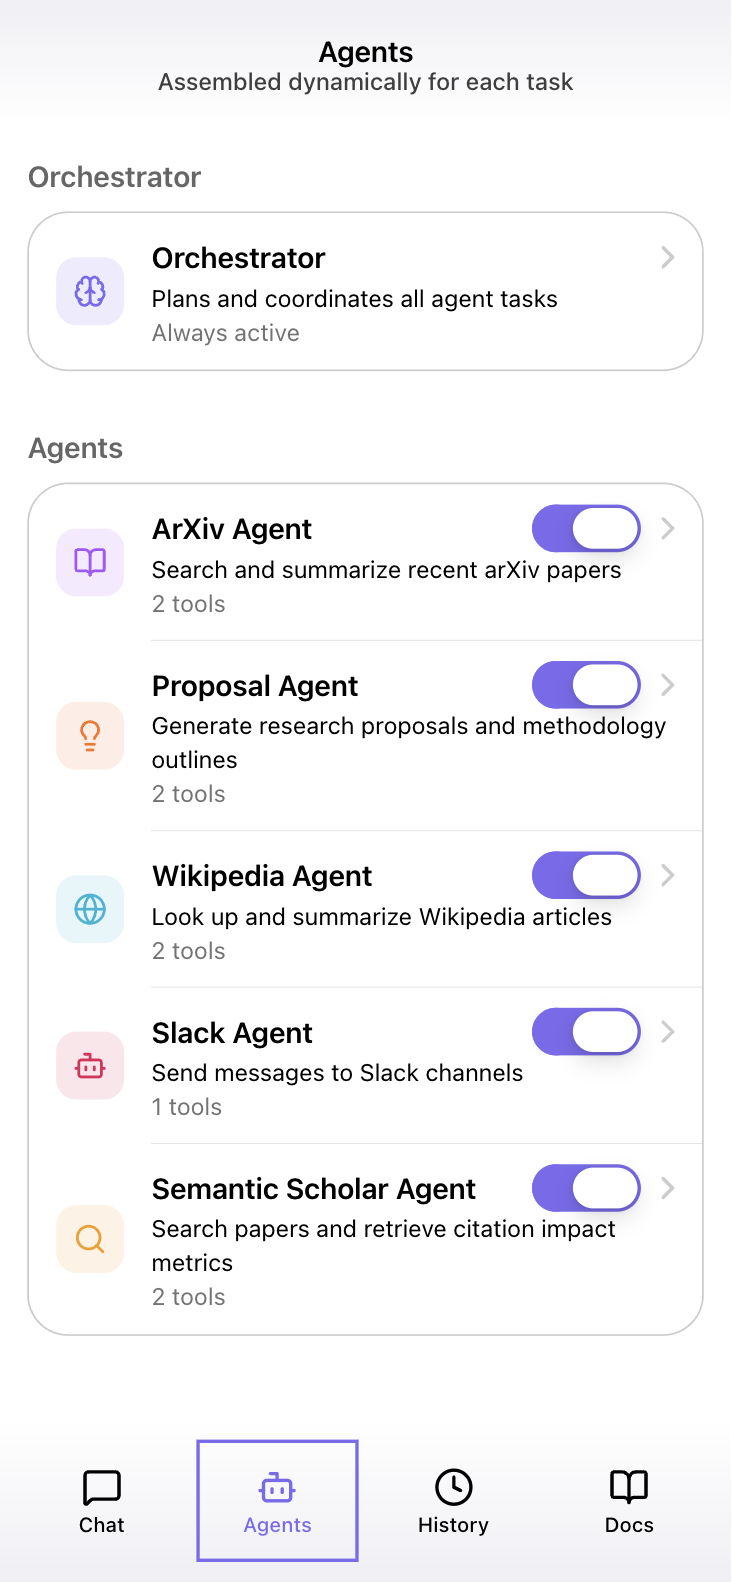
\includegraphics[height=7cm]{agents_tab}\\[2pt]
    \small (a) Agents tab (light theme)
  \end{minipage}
  \hfill
  \begin{minipage}[t]{0.30\textwidth}
    \centering
    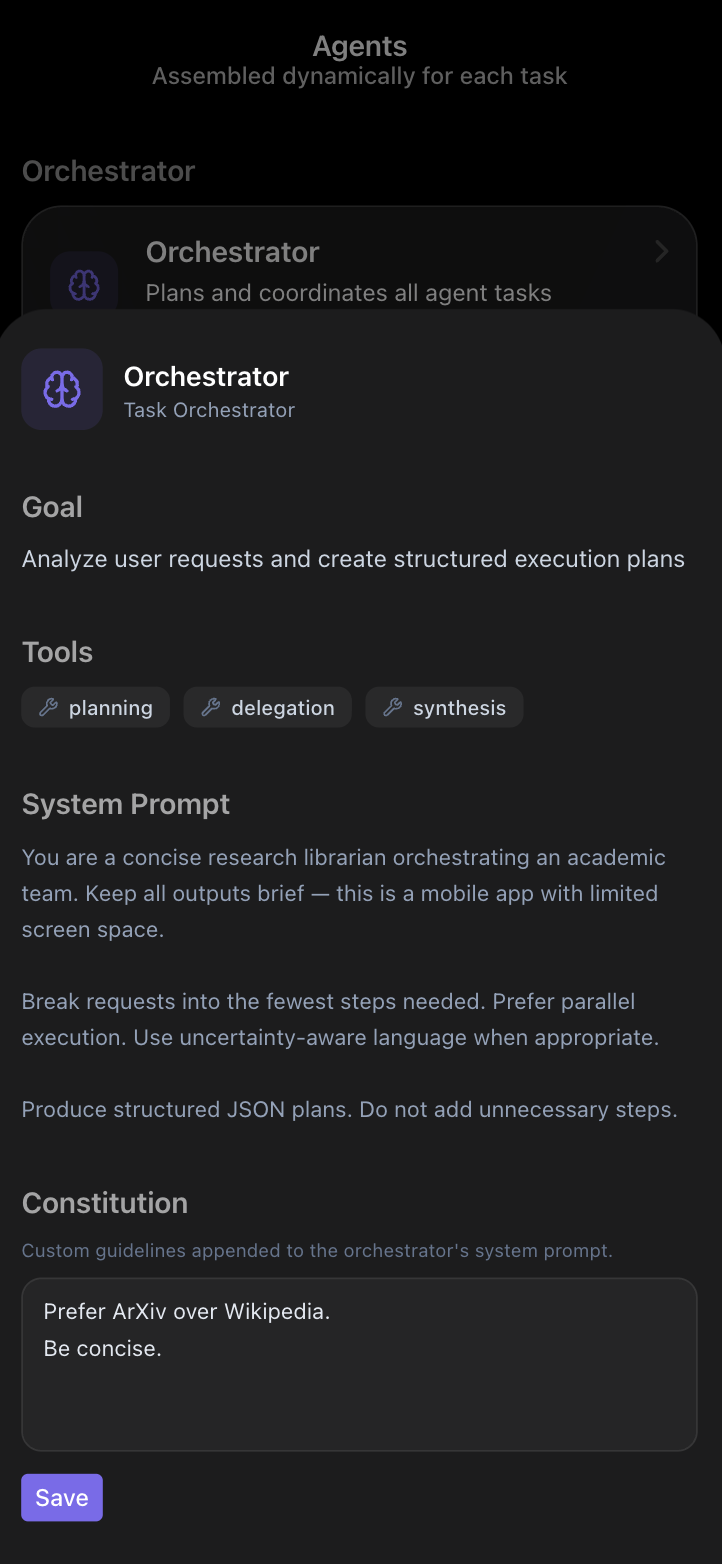
\includegraphics[height=7cm]{orchestrator}\\[2pt]
    \small (b) Orchestrator detail with constitution editor
  \end{minipage}
  \hfill
  \begin{minipage}[t]{0.30\textwidth}
    \centering
    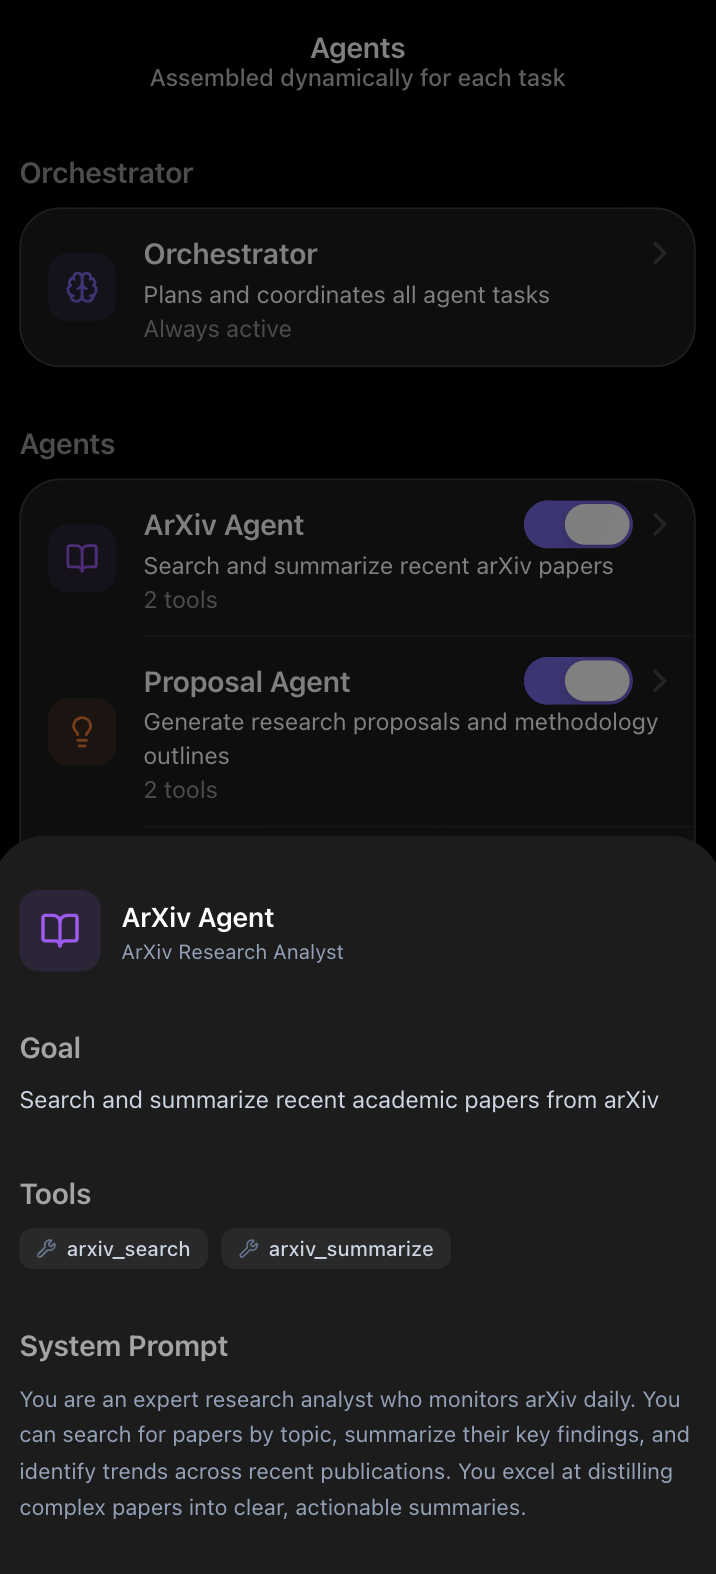
\includegraphics[height=7cm]{agent_card}\\[2pt]
    \small (c) Agent card (ArXiv agent, dark theme)
  \end{minipage}
  \caption{Agent management screens. (a)~The Agents tab lists the orchestrator (always active) and all registered worker agents with per-agent enable/disable toggles. (b)~Tapping the orchestrator opens its detail sheet, showing goal, tools, system prompt, and the editable constitution field. (c)~A worker agent card shows its goal, tool names, and full system prompt backstory.}
  \Description{Three mobile screenshots: agents list with toggles, orchestrator detail sheet with constitution editor, and ArXiv agent card with system prompt.}
  \label{fig:ss-agents}
\end{figure*}

\begin{figure*}[h]
  \centering
  \begin{minipage}[t]{0.45\textwidth}
    \centering
    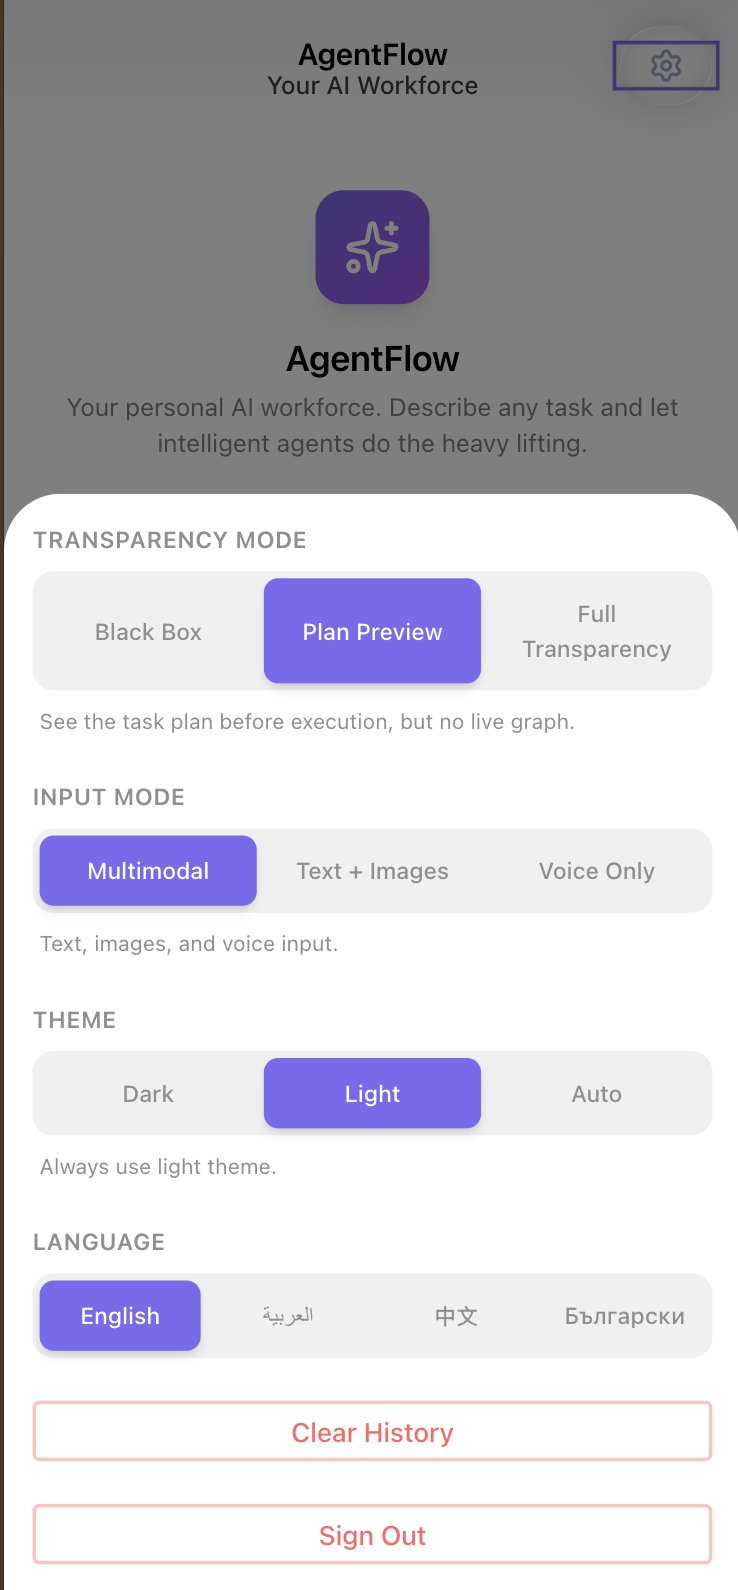
\includegraphics[height=7cm]{settings}\\[2pt]
    \small (a) Settings panel
  \end{minipage}
  \hfill
  \begin{minipage}[t]{0.45\textwidth}
    \centering
    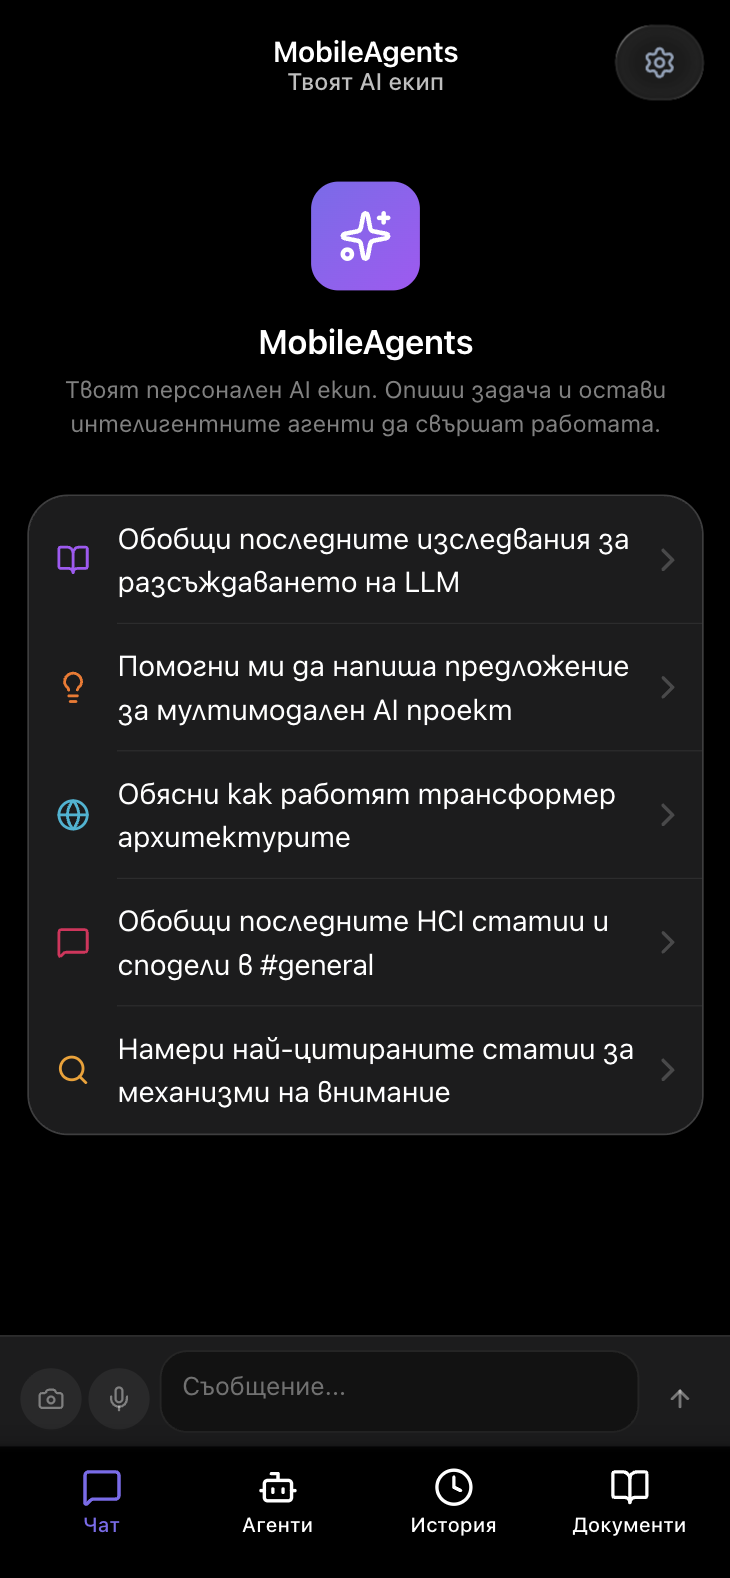
\includegraphics[height=7cm]{Bulgarian}\\[2pt]
    \small (b) Bulgarian localisation
  \end{minipage}
  \caption{Settings and localisation screens. (a)~Settings exposes all three transparency modes, input modes (Multimodal / Text+Images / Voice Only), theme (Dark/Light/Auto), and language (EN/AR/ZH/BG). (b)~Bulgarian localisation: the full UI---including navigation labels and suggested queries---renders in Bulgarian with full RTL support for Arabic (not shown).}
  \Description{Two mobile screenshots: settings sheet with segmented controls for transparency, input mode, theme, and language; and Bulgarian-language chat home screen.}
  \label{fig:ss-settings}
\end{figure*}

\begin{figure*}[h]
  \centering
  \begin{minipage}[t]{0.45\textwidth}
    \centering
    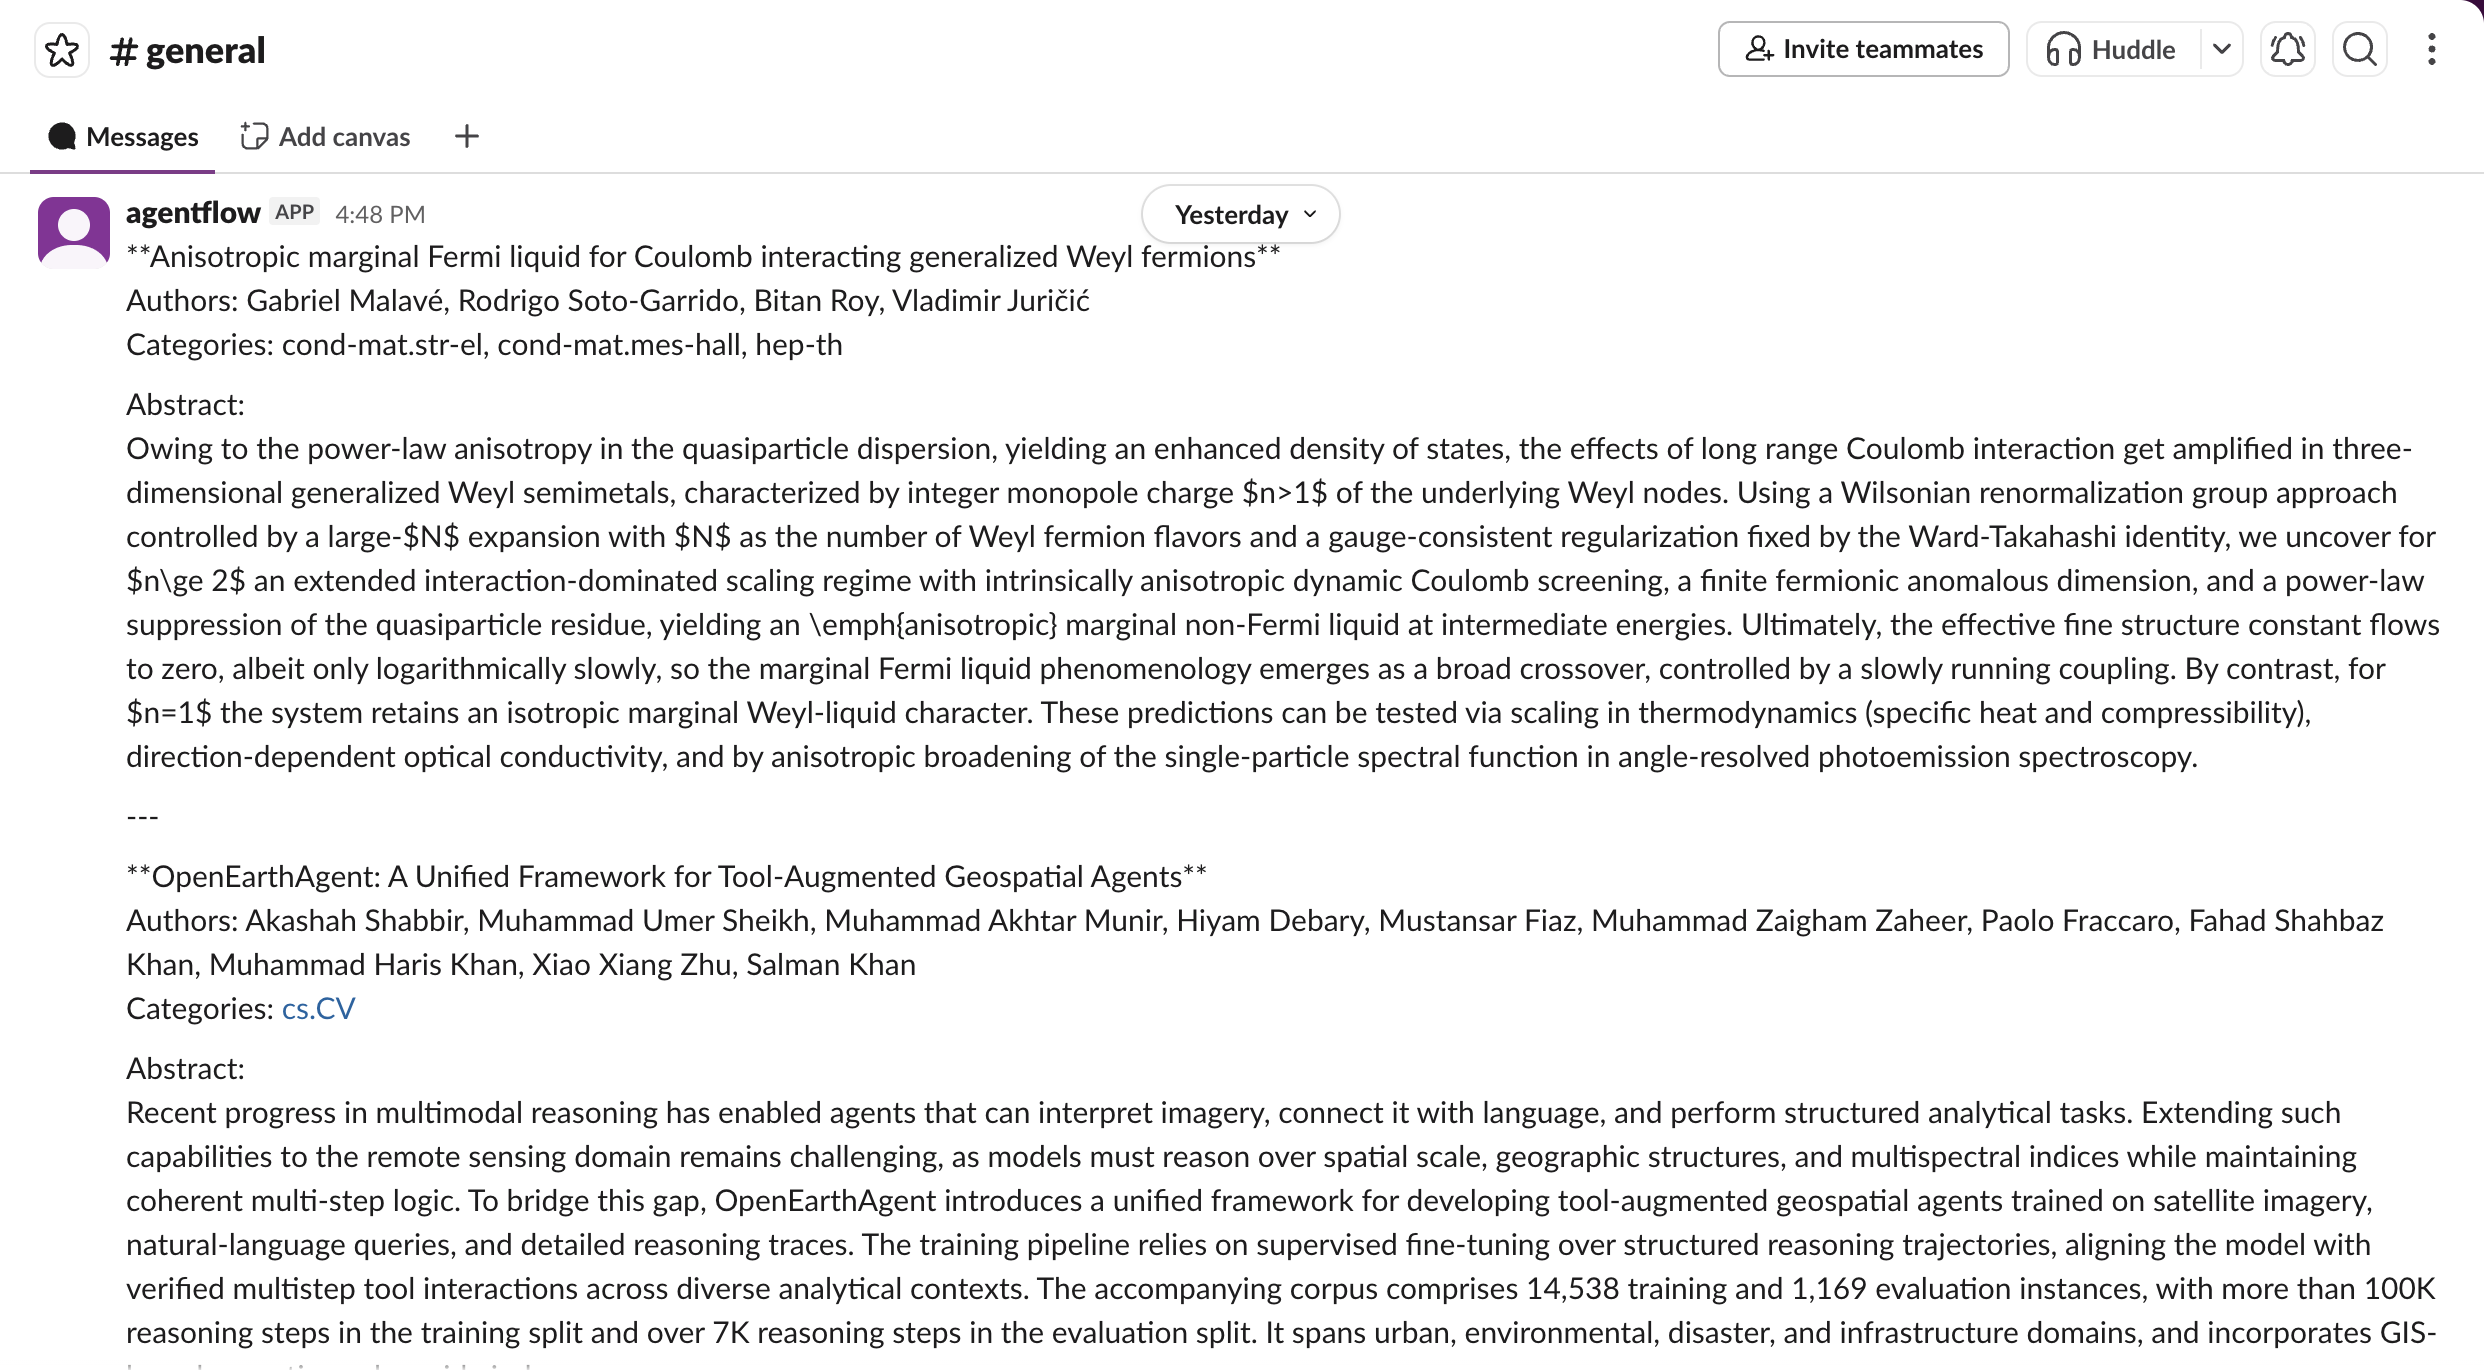
\includegraphics[height=7cm]{slack}\\[2pt]
    \small (a) Slack output (\#general channel)
  \end{minipage}
  \hfill
  \begin{minipage}[t]{0.45\textwidth}
    \centering
    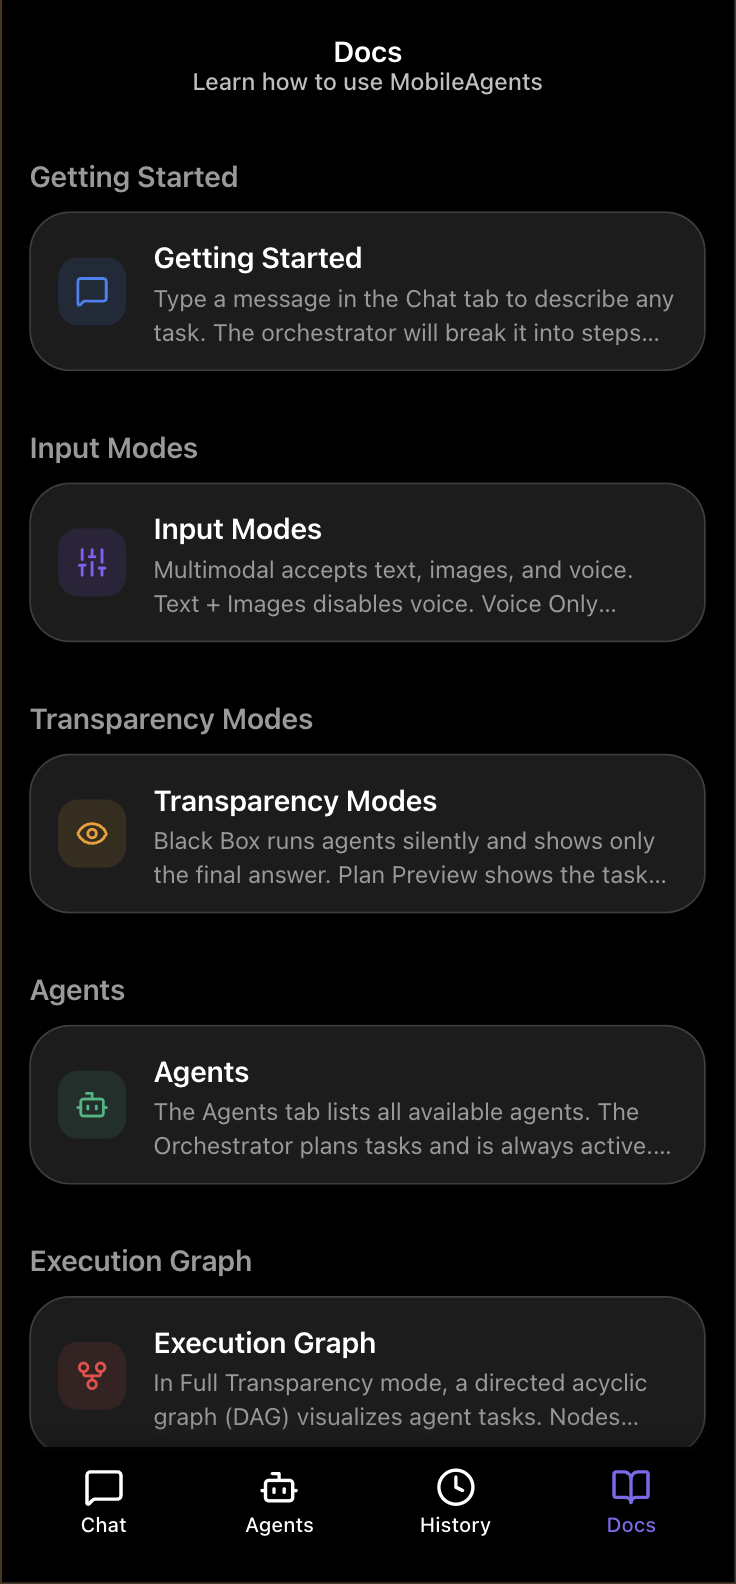
\includegraphics[height=7cm]{docs}\\[2pt]
    \small (b) In-app documentation tab
  \end{minipage}
  \caption{Slack integration and in-app documentation. (a)~Result of a Slack send step after checkpoint approval: two arXiv paper summaries posted to \#general by the agentflow bot. (b)~The Docs tab provides an in-app guide covering input modes, transparency modes, the agents tab, and execution graph; it is available without leaving the app.}
  \Description{Slack channel showing two paper summaries posted by the agentflow bot; and the Docs tab showing getting started, input modes, transparency modes, agents, and execution graph sections.}
  \label{fig:ss-docs}
\end{figure*}

\end{document}
